\documentclass[UTF8]{ctexart}

\usepackage[hidelinks]{hyperref}
\usepackage{fancyhdr}
\usepackage{graphicx}
\usepackage{float}
\usepackage{amsmath}
\usepackage{amssymb}
\usepackage{latexsym}

\usepackage{xcolor}     %高亮使用的颜色
\definecolor{commentcolor}{RGB}{85,139,78}
\definecolor{stringcolor}{RGB}{206,145,108}
\definecolor{keywordcolor}{RGB}{34,34,250}
\definecolor{backcolor}{RGB}{220,220,220}

\usepackage{accsupp}    
\newcommand{\emptyaccsupp}[1]{\BeginAccSupp{ActualText={}}#1\EndAccSupp{}}

\usepackage{listings}
\lstset{                        %高亮代码设置
    language=python,                    %Python语法高亮
    linewidth=1.3\linewidth,            %列表list宽度
    %basicstyle=\ttfamily,              %tt无法显示空格
    commentstyle=\color{commentcolor},  %注释颜色
    keywordstyle=\color{keywordcolor},  %关键词颜色
    stringstyle=\color{stringcolor},    %字符串颜色
    %showspaces=true,                   %显示空格
    %numbers=left,                       %行数显示在左侧
    %numberstyle=\tiny\emptyaccsupp,     %行数数字格式
    %numbersep=5pt,                      %数字间隔
    frame=single,                       %加框
    framerule=0.1pt,                      %不划线
    escapeinside=@@,                    %逃逸标志
    emptylines=1,                       %
    xleftmargin=0.2em,                    %list左边距
    %backgroundcolor=\color{backcolor},  %列表背景色
    tabsize=4,                          %制表符长度为4个字符
    gobble=4                            %忽略每行代码前4个字符
    }
\begin{document}

\begin{figure}[H]
 \centering
  
\includegraphics[width=8cm,height=8cm]{logo.jpg}

\end{figure}

\begin{center}
~\\
~\\
~\\
~\\
\textbf{\Huge \Huge  数值计算实验报告}\\
\large
~\\
~\\
~\\
~\\
~\\
~\\
赵晓辉 \quad 2017级数据班 \quad 201700150139  \\
指导教师:刘保东教授
\end{center}
\thispagestyle{empty}
\newpage


\tableofcontents
\thispagestyle{empty}
\newpage
\setcounter{page}{1}
\pagestyle{empty} 
\section*{Summary}%摘要
数值计算指有效使用数字计算机求数学问题近似解的方法与过程,以及由相关理论构成的学科。主要研究如何用计算机能够更好的解决数学问题。

在数值计算的课程实验中,我们使用 PYTHON 对数学领域的常用算法进行了学习和编程实现,并进行了误差分析。内容包括线性方程组的求解、插值与拟合、微分与积分等内容,编写了若干经典算法,对课堂上讲的内容有了更深刻的理解。

进行完实验的学习之后,我们对计算机和数学之间的联系理解的更加透彻,为以后的科研之路打下了良好的基础。

本实验报告由latex编写,其中所有代码开源于

\href{https://github.com/zxh991103/NumericalCalculation/}{https://github.com/zxh991103/NumericalCalculation/}


\newpage


\section{第一章误差理论}

\subsection{problem 1}
根据以下方法构造算法和 MATLAB 程序,以便精确计算所有情况下的二次方程的根,包括$|b| \approx \sqrt {b^2-4ac} $的情况。


设$ a \not= 0 ,b^2-4ac > 0 $且有方程$ ax^2+bx+c=0$


\begin{equation}
\begin{array}{rcl}
x_1=\frac{-b+\sqrt{b^2-4ac}}{2a} , x_2=\frac{-b-\sqrt{b^2-4ac}}{2a}& & { }\\
\end{array}
\end{equation}

公式(1)(2)等价于下列公式

\begin{equation}
\begin{array}{rcl}
x_1=\frac{-2c}{b+\sqrt{b^2-4ac}} , x_2=\frac{-2c}{b-\sqrt{b^2-4ac}}& & { }\\
\end{array}
\end{equation}

当$b>0$的时候使用公式(1)计算$ x_1$ ,使用公式(2)计算$ x_2$。


当$b<0$的时候使用公式(1)计算$ x_2$ ,使用公式(2)计算$ x_1$。

求解方程如下:

(a)$ x^2-1000.001x+1=0$

(b)$ x^2-10000.0001x+1=0$

(c)$ x^2-100000.00001x+1=0$

(d)$ x^2-1000000.000001x+1=0$

结果如下:

(a)$ x_1=1000.0000000236469 , x_2=0.0009999999999763531$

(b)$ x_1=9999.999979772838 , x_2=0.00010000000020227162$

(c)$ x_1=99999.96614643588 , x_2=1.0000003385357559\times 10^{-5}$

(d)$ x_1=999992.38556461 , x_2=1.00000761449337\times 10^{-6}$										

由于计算机的发展和精确度的提高,使用题目中的方法的python实现和普通的二次求根公式进行计算的结果相差不大。

python实现代码如下:
\begin{lstlisting}

	def f_11(a, b, c):
    t = pow(b * b - 4 * a * c, 0.5)
    x1 = (-b + t) / (2 * a)
    return x1

	def f_12(a, b, c):
	    t = pow(b * b - 4 * a * c, 0.5)
	    x2 = (-b - t) / (2 * a)
	    return x2


	def f_21(a, b, c):
	    t = pow(b * b - 4 * a * c, 0.5)
	    x1 = (-2 * c) / (b + t)
	    return x1

	def f_22(a, b, c):
	    t = pow(b * b - 4 * a * c, 0.5)
	    x2 = (-2 * c) / (b - t)
	    return x2



	l = [[1, -1000.001, 1],
	     [1, -10000.0001, 1],
	     [1, -100000.00001, 1],
	     [1, -1000000.000001, 1]]

	for k in l:
	    if k[1]<0:
	        print(f_21(k[0],k[1],k[2]),f_12(k[0],k[1],k[2]))
	    else:
	        print(f_11(k[0], k[1], k[2]), f_22(k[0], k[1], k[2]))
    

	
\end{lstlisting}

\subsection{problem 2}
对下列 3 个差分方程计算出前十个数值近似值。在每种情况下引入一个小的初始误差。如果没有初始误差,则每个差分方程将生成序列${ (\frac{1}{2})_{n=1}^{\infty} }$ 。

构造误差表和误差图。

(a)$r_0=0.994,r_n=\frac{1}{2} r_{n-1}$,其中$n=1,2, \cdots$

(b)$p_0=1,p_1=0.497,p_n=\frac{3}{2} p_{n-1} - \frac{1}{2} p_{n-2}$,其中$n=2,3, \cdots$

(c)$q_0=1,q_1=0.497,q_n=\frac{5}{2} q_{n-1} - q_{n-2}$,其中$n=2,3, \cdots$

利用如下python代码根据题目中的公式进行迭代。
\begin{lstlisting}

	import numpy as np
	r=[0.994]
	p=[1,0.497]
	q=[1,0.497]
	x=[1]
	for i in range(20):
	    t=0.5*r[i]
	    r.append(t)
	    t=1.5*p[i+1]-0.5*p[i]
	    p.append(t)
	    t=2.5*q[i+1]-0.5*q[i]
	    q.append(t)
	    t=0.5*x[i]
	    x.append(t)
	print(q[2])
	x=x[0:11]
	r=r[0:11]
	p=p[0:11]
	q=q[0:11]

	x_r_p_q=np.array([x,r,p,q]).T

	print(x_r_p_q)


	t=[i for i in range(11)]

	x_r=[(i[0]-i[1]) for i in x_r_p_q]
	x_p=[(i[0]-i[2]) for i in x_r_p_q]
	x_q=[-(i[0]-i[3]) for i in x_r_p_q]

	import matplotlib.pyplot as plt

	plt.plot(t,x_r)
	plt.scatter(t,x_r)
	plt.show()

	plt.plot(t,x_p)
	plt.scatter(t,x_p)
	plt.show()

	plt.plot(t,x_q)
	plt.scatter(t,x_q)
	plt.show()

	
\end{lstlisting}


得到$ r_n $、$ p_n$ 、$ q_n $结果数值如下:


\begin{table}[H]
\caption{x、r、p、q数值表}
\begin{tabular}{|l|l|l|l|l|}
\hline

n & x & r & p & q \\ \hline
0 & 1 & 0.994 & 1 & 1 \\ \hline
1 & 0.5 & 0.497 & 0.497 & 0.497 \\ \hline
2 & 0.25 & 0.2485 & 0.2455 & 0.7425 \\ \hline
3 & 0.125 & 0.12425 & 0.11975 & 1.60775 \\ \hline
4 & 0.0625 & 0.062125 & 0.056875 & 3.648125 \\ \hline
5 & 0.03125 & 0.0310625 & 0.0254375 & 8.3164375 \\ \hline
6 & 0.015625 & 0.01553125 & 0.00971875 & 18.96703125 \\ \hline
7 & 0.0078125 & 0.007765625 & 0.001859375 & 43.25935937 \\ \hline
8 & 0.00390625 & 0.003882813 & -0.002070312 & 98.66488281 \\ \hline
9 & 0.001953125 & 0.001941406 & -0.004035156 & 225.0325273 \\ \hline
10 & 0.000976563 & 0.000970703 & -0.005017578 & 513.248877 \\ \hline

\end{tabular}
\end{table}

\begin{table}[H]

\caption{差值表}
\begin{tabular}{|l|l|l|l|}
\hline

n & x-r & x-p & x-q \\ \hline
0 & 0.006 & 0 & 0 \\ \hline
1 & 0.003 & 0.003 & -0.003 \\ \hline
2 & 0.0015 & 0.0045 & 0.4925 \\ \hline
3 & 0.00075 & 0.00525 & 1.48275 \\ \hline
4 & 0.000375 & 0.005625 & 3.585625 \\ \hline
5 & 0.0001875 & 0.0058125 & 8.2851875 \\ \hline
6 & 0.00009375 & 0.00590625 & 18.95140625 \\ \hline
7 & 0.000046875 & 0.005953125 & 43.25154687 \\ \hline
8 & 0.0000234375 & 0.005976562 & 98.66097656 \\ \hline
9 & 0.00001171875 & 0.005988281 & 225.0305742 \\ \hline
10 & 0.000005859375 & 0.005994141 & 513.2479004 \\ \hline

\end{tabular}
\end{table}



误差$ x_n-r_n$、$ x_n-p_n$、$ x_n-q_n$的分布图如下:

\begin{figure}[H]
 \centering
  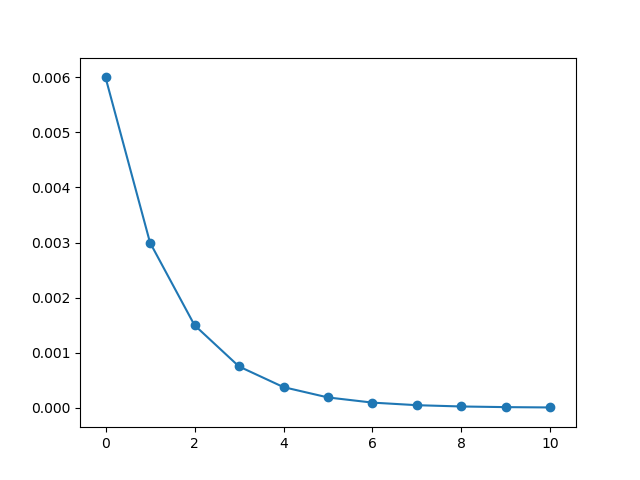
\includegraphics[width=10cm,height=9cm]{1-2-1.png}
  \caption{xn-rn误差变化图}
\end{figure}


\begin{figure}[H]
 \centering
  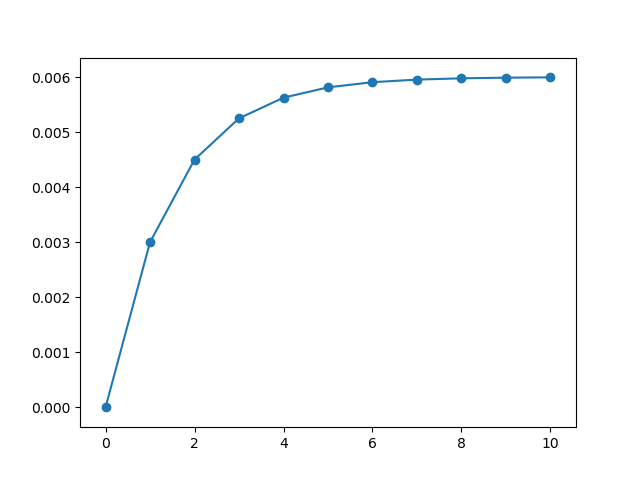
\includegraphics[width=10cm,height=9cm]{1-2-2.png}
  \caption{xn-pn误差变化图}
\end{figure}



\begin{figure}[H]
 \centering
  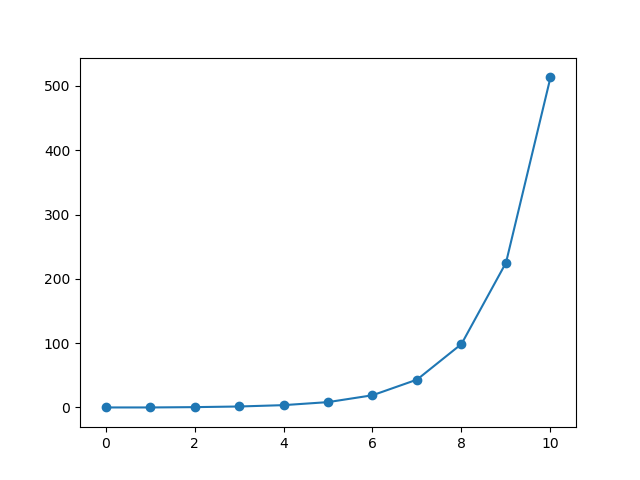
\includegraphics[width=10cm,height=9cm]{1-2-3.png}
  \caption{xn-qn误差变化图}
\end{figure}




\newpage
\subsection{作业}
~\\
2.完成下列计算:

$ \int_{0}^{1 / 4} e^{x^{2}} d x  \approx \int_{0}^{1 / 4}\left(1+x^{2}+\frac{x^{4}}{2 !}+\frac{x^{6}}{3 !}\right) d x = \hat{p}$


指出在这种情况下会出现哪种类型的误差,并将计算结果与真实值p=0.2553074606进行比较。


$\begin{aligned} \int_{0}^{1 / 4} e^{x^{2}} d x & \approx \int_{0}^{1 / 4}\left(1+x^{2}+\frac{x^{4}}{2 !}+\frac{x^{6}}{3 !}\right) d x \\ 
&=\left(x+\frac{x^{3}}{3}+\frac{x^{5}}{5(2 !)}+\frac{x^{7}}{7(3 !)}\right)_{x=0}^{x=1 / 4} \\ 
&=\frac{1}{4}+\frac{1}{19^{2}}+\frac{1}{10240}+\frac{x^{2}}{688128} \\ 
&=\frac{292807}{1146880} \approx 0.255307428=\hat{p} 
\end{aligned}$


$ | \hat{p}-p |=3.2599999977289684 \times 10^{-8}$

误差分为2个部分:

\quad1.使用泰勒公式余项带来的误差。

\quad2.浮点数运算带来的误差


~\\ 
~\\
~\\

5.有时利用三角或代数恒等式,重新排列函数中的项,可以避免精度损失。求下列函数的等价公式,以避免精度损失。

(a)ln(x+1)-ln(x),其中x较大。

(b)$ \sqrt{x^2+1} - x$,其中x较大。

(c)$ cos^2 (x) - sin^2 (x)$,其中x$\approx \frac{\pi}{4}$ 

(d)$ \sqrt{\frac{1+cos(x)}{2}} $,其中x$\approx \pi$ 

answer:


\quad (a)ln(x+1)-ln(x)=ln $ \frac{x+1}{x}$

\quad (b)$ \sqrt{x^2+1} - x = \frac{1}{\sqrt{x^2+1}+x}  $

\quad (c)$ cos^2 (x) - sin^2 (x) = cos (2x)$

\quad (d)$ \sqrt{\frac{1+cos(x)}{2}} = \sqrt\frac{{1+2cos^2 \frac{x}{2} -1}}{2}  = cos(\frac{x}{2})$



~\\ 
~\\
~\\

8.讨论下列计算过程中的误差传播

(a)三个数的和:

\quad \quad p+q+r=$(\hat{p}+\epsilon_{p})+(\hat{q}+\epsilon_{q})+(\hat{r}+\epsilon_{r}) $


(b)两个数的商:$ \frac{p}{q} = \frac{\hat{p}+\epsilon_{p}}{\hat{q}+\epsilon_{q}}$


(c)三个数的积:

\quad \quad pqr=$(\hat{p}+\epsilon_{p})(\hat{q}+\epsilon_{q})(\hat{r}+\epsilon_{r}) $


answer:


(a)误差传播为:

 $ (p+q+r)-(\hat{p}+\hat{q}+\hat{r}) $~\\
 \quad$=(\hat{p}+\epsilon_{p})+(\hat{q}+\epsilon_{q})+(\hat{r}+\epsilon_{r})-(\hat{p}+\hat{q}+\hat{r})$~\\ 
\quad$=\epsilon_{p}+\epsilon_{q}+\epsilon_{r} $

(b)误差传播为:

 $ (\frac{p}{q})-(\frac{\hat{p}}{\hat{q}}) $~\\
 \quad$= (\frac{\hat{p}+\epsilon_{p}}{\hat{q}+\epsilon_{q}})-(\frac{\hat{p}}{\hat{q}})$~\\ 
\quad$=\frac{\hat{p}}{\hat{q}} + \frac{\epsilon_{p} - \frac{p}{q}\epsilon_{q} }{q+\epsilon_{p}} -(\frac{\hat{p}}{\hat{q}})$~\\
\quad $ = \frac{\epsilon_{p} - \frac{p}{q}\epsilon_{q} }{q+\epsilon_{p}}$

当$ 1<|\hat{q}|<|\hat{p}|$时,误差较大。

(c)误差传播为:

$\begin{aligned} p q r=&\left(\hat{p}+\epsilon_{p}\right)\left(\hat{q}+\epsilon_{q}\right)\left(\hat{r}+\epsilon_{r}\right) \\=& \hat{p} \hat{q} \hat{r}+\hat{p} \hat{r} \epsilon_{q}+\hat{q} \hat{r} \epsilon_{p}+\hat{p} \hat{q} \epsilon_{r}+\hat{r} \epsilon_{p} \epsilon_{q}+\hat{q} \epsilon_{p} \epsilon_{r}+\hat{p} \epsilon_{q} \epsilon_{r}+\epsilon_{p} \epsilon_{q} \epsilon_{r} \\=& \hat{p} \hat{q} \hat{r}+\left(\hat{p} \hat{r} \epsilon_{q}+\hat{q} \hat{r} \epsilon_{p}+\hat{p} \hat{q} \epsilon_{r}\right) \\ &+\left(\hat{r} \epsilon_{p} \epsilon_{q}+\hat{q} \epsilon_{p} \epsilon_{r}+\hat{p} \epsilon_{q} \epsilon_{r}\right)+\epsilon_{p} \epsilon_{q} \epsilon_{r} \end{aligned}$

若$ \hat{q}.\hat{p}.\hat{r}$ 的绝对值较大,误差较大


~\\
~\\
~\\


11.设有泰勒展开式:

\quad \quad $ cos(h)=1-\frac{h^2}{2!} + \frac{h^4}{4!} +  \boldsymbol{O} (h^5)$

和

\quad \quad $ sin(h)=h-\frac{h^3}{3!} + \frac{h^5}{5!} +  \boldsymbol{O} (h^7)$

判定它们的和与积的近似阶。

answer:

$\begin{aligned} \cos (h)+\sin (h) &=1+h-\frac{h^{2}}{2}-\frac{h^{3}}{6}+\frac{h^{4}}{24}+\boldsymbol{O}\left(h^{5}\right) \\ \cos (h) \sin (h) &=h-\frac{2 h^{3}}{3}+\frac{2 h^{5}}{15}+\boldsymbol{O}\left(h^{7}\right) \end{aligned}$

$1. cos(h)\times sin(h)=\frac{1}{2} sin(2h) $


$2. \left(1-\frac{h^{2}}{2}+\frac{h^{4}}{24}\right)\left(h-\frac{h^{3}}{6}+\frac{h^{5}}{120}\right)=h-\frac{2 h^{3}}{3}+\frac{2 h^{5}}{15}-\frac{h^{7}}{90}+\frac{h^{9}}{2880}$




\newpage
\section{第二章非线性方程求根}



\subsection{problem 1}


求方程$2 x^{2}+x-15=0$的正根近似值,分别利用如下三种格式编程计算:

(a)
$x_{k+1}=15-x_{k}^{2}, k=0,1,2, \cdots$取初始值$ x_0 =2$

(b)
$ x_{k+1}=\frac{15}{2 x_k+1}, k=0,1,2, \cdots$取初始值$ x_0 =2$

(c)
$ x_{k+1}=x_{k}-\frac{2 x_{k}^{2}+x_{k}-15}{4 x_{k}+1}, k=0,1,2, \cdots$取初始值$ x_0 =2$

依次计算$x_{1}, x_{2}, \cdots, x_{k}, \cdots$并作图观察解的稳定性、收敛性,并分析其原因。


\subsubsection{problem 1.1}



(a)python实现代码如下:


\begin{lstlisting}
	import numpy as np
	import matplotlib.pyplot as plt
	N=4


	l1=[2]
	for i in range(1,N):
	    l1.append(15-pow(l1[i-1],2))

	l2=[]
	for i in range(N):
	    l2.append(i)

	x=np.asanyarray(l2)
	y=np.asanyarray(l1)

	plt.scatter(x, y)
	plt.show()



\end{lstlisting}

\begin{figure}[H]
 \centering
  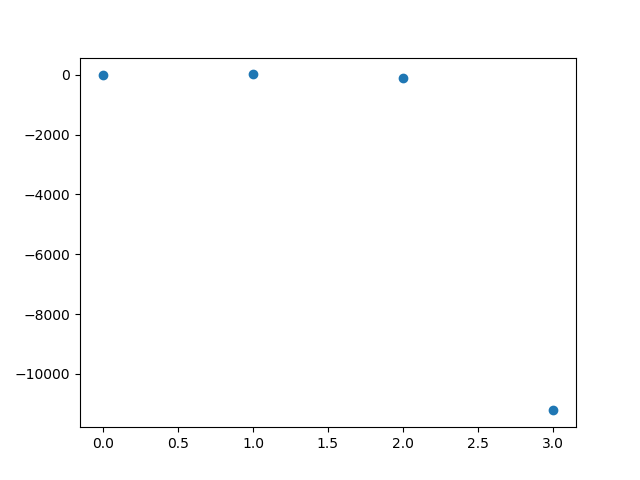
\includegraphics[width=10cm,height=9cm]{2-1-1.png}
  \caption{xk图(a)}
\end{figure}



使用此种方法,获得的解不收敛,$$x_0=2,x_1=11,x_2=-106$$然后递减,永不收敛。


\subsubsection{problem 1.2}

(b)python实现代码如下:

\begin{lstlisting}

	import numpy as np
	import matplotlib.pyplot as plt
	N=100


	l1=[2]
	for i in range(1,N):
	    l1.append(15/(2*l1[i-1]+1))

	l2=[]
	for i in range(N):
	    l2.append(i)

	x=np.asanyarray(l2)
	y=np.asanyarray(l1)

	plt.scatter(x, y)
	plt.show()
\end{lstlisting}

\begin{figure}[H]
 \centering
  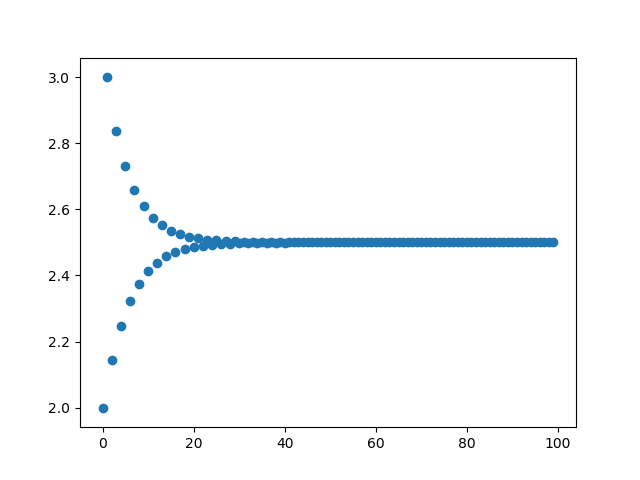
\includegraphics[width=10cm,height=9cm]{2-1-2.png}
  \caption{xk图(b)}
\end{figure}

该方法收敛相(c)较慢。
$$
x_{k+1} \times (2x_k+1)=15
$$


$$
2x_{k+1}x_{k}+x_{k+1}-15=0
$$

当$x>5$时:

$$
g^{\prime} (x)=\frac{-30}{(2x_k+1)^2}
$$


$$
|g^{\prime} (x)|<1
$$



\subsubsection{problem 1.3}



(c)python实现代码如下:
\begin{lstlisting}

	import numpy as np
	import matplotlib.pyplot as plt
	N=10


	l1=[2]
	for i in range(1,N):
	    l1.append(l1[i-1] - (2*pow(l1[i-1],2)+l1[i-1]-15)/(4*l1[i-1]+1))

	l2=[]
	for i in range(N):
	    l2.append(i)

	x=np.asanyarray(l2)
	y=np.asanyarray(l1)

	plt.scatter(x, y)
	plt.show()
\end{lstlisting}

\begin{figure}[H]
 \centering
  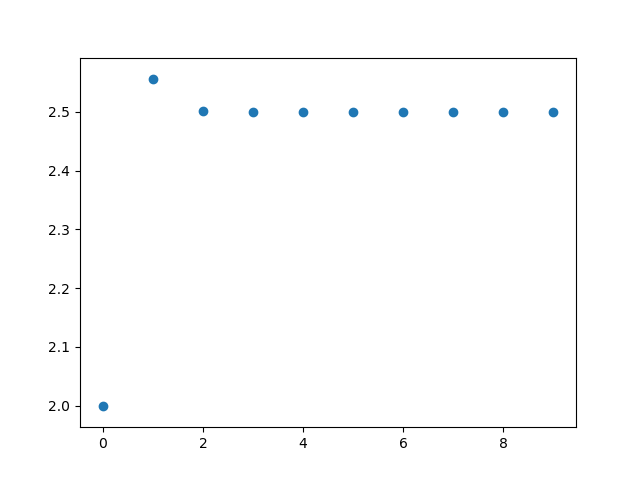
\includegraphics[width=10cm,height=9cm]{2-1-3.png}
  \caption{xk图(c)}
\end{figure}

$$
-(x_{k+1}-x_{k})(4x_k+1)=2{x_k}^2+x_k-15
$$

当$$lim_{k->\infty}x_k=x_{k+1}$$


$$
0=2{x_k}^2+x_k-15
$$


当$x>5$时:

$$
g^{\prime} (x)=4\frac{2x^2+x+1}{16x^2+8x+1}
$$


$$
|g^{\prime} (x)|<1
$$





\subsection{problem 2}
证明方程$2-3x-sin(x)=0 $在(0,1)内有且有一个实根,使用二分法求误差不大于0.0005的根,及其需要的迭代次数。

python实现代码如下:

\begin{lstlisting}
	import math
	def f(x):
	    return 2-3*x-math.sin(x)
	
	print('prove:f(0)*f(1)=',f(0)*f(1),'<0')

	x1=0
	x2=1
	i=0
	while x2-x1>0.000005:
	    i+=1
	    x=(x1+x2)/2
	    if f(x)*f(x1)<=0:
	        x2=x
	    else:
	        x1=x

	print(x1)
	print(i)

\end{lstlisting}

证明:

\begin{math}
f(0) \cdot f(1)= -3.682941969615793 <0\\
f^{'}\left( x\right) =-3-\cos x\\
-\cos x\leq 1 \\
f^{'}\left( x\right)  <0
\end{math}

f(x)单调递减


使用二分法误差不大于0.0005的根为$ 0.50530624389648440$

迭代次数$18$

\subsection{problem 3}

利用牛顿法求解方程:
$ \frac{1}{2}+\frac{1}{4} x^{2}-x \sin x-\frac{1}{2} \cos 2 x=0$
分别取$ x_{0}=\frac{\pi}{2}, 5 \pi, 10 \pi$ ,使得精度不超过$ 10^{-5}$比较初值对计算结果的影响
\begin{lstlisting}
	import math
	import numpy as np
	from sympy import *
	import matplotlib.pyplot as plt
	def f(x):
	    return 0.5+0.25*pow(x,2)-x*math.sin(x)-0.5*math.cos(2*x)

	delta = 0.01

	def f_1(x):
	    return (f(x+delta)-f(x))/delta

	def f_2(x):
	    return (f_1(x+delta)-f_1(x))/delta


	def g(x):
	    return x-f(x)/f_1(x)





	def cal(x0):
	    res=[0,x0]
	    t1=0
	    t2=x0
	    while ( abs( t1-t2 ) > pow(10,-5) ):
	        t1=t2
	        t2=g(res[len(res)-1])
	        res.append(t2)
	    return res


	x0=math.pi/2
	x1=math.pi*5
	x2=math.pi*10

	r0=cal(x0)
	r1=cal(x1)
	r2=cal(x2)

	y0=[]
	y1=[]
	y2=[]

	for i in range(len(r0)):
	    y0.append(i)

	for i in range(len(r1)):
	    y1.append(i)

	for i in range(len(r2)):
	    y2.append(i)

	print(r0[-1],r1[-1],r2[-1])
	x=np.asanyarray(y0)
	y=np.asanyarray(r0)
	plt.plot(x,y)
	plt.scatter(x, y)
	plt.savefig('2-3-0.png')
	plt.show()
	x=np.asanyarray(y1)
	y=np.asanyarray(r1)
	plt.plot(x,y)
	plt.scatter(x, y)
	plt.savefig('2-3-1.png')
	plt.show()

	x=np.asanyarray(y2)
	y=np.asanyarray(r2)
	plt.plot(x,y)
	plt.scatter(x, y)
	plt.savefig('2-3-2.png')
	plt.show()

\end{lstlisting}

\begin{figure}[H]
 \centering
  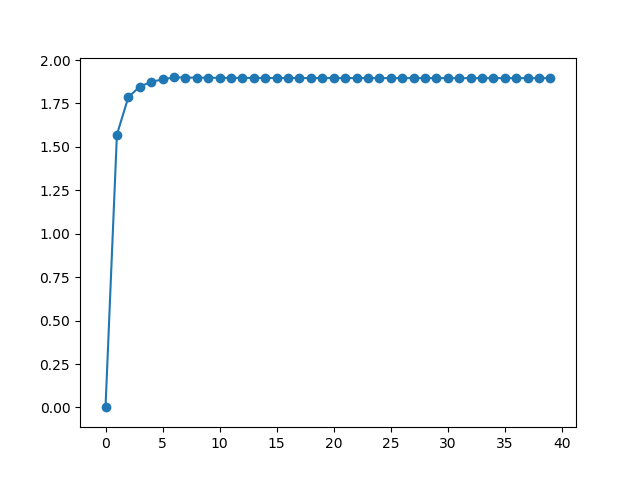
\includegraphics[width=10cm,height=9cm]{2-3-0.png}
  \caption{x0图}
\end{figure}


\begin{figure}[H]
 \centering
  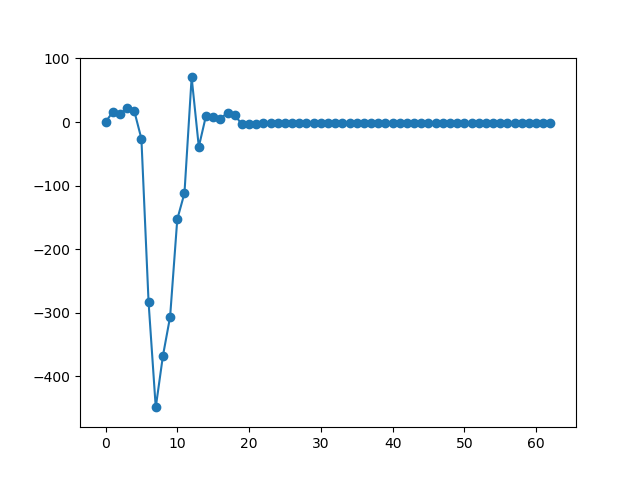
\includegraphics[width=10cm,height=9cm]{2-3-1.png}
  \caption{x1图}
\end{figure}

\begin{figure}[H]
 \centering
  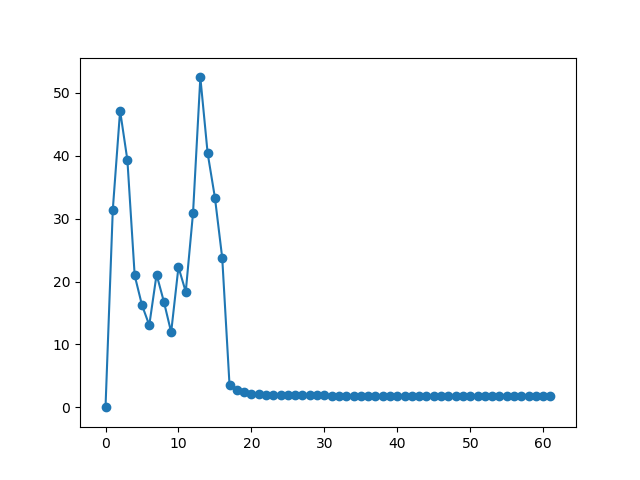
\includegraphics[width=10cm,height=9cm]{2-3-2.png}
  \caption{x2图}
\end{figure}

收敛过程不同,最后分别收敛到1.8958096931257646,-1.8951889600105052,1.8958113494649107


\subsection{problem 4}
python实现代码如下:
\begin{lstlisting}

	import math

	def f(x):
	    return 5*x-math.exp(x)	
\end{lstlisting}
\begin{lstlisting}%'二分结果:',

	x1=0
	x2=1
	while x2-x1>0.0001:
	    x=(x1+x2)/2
	    if f(x)*f(x1)<=0:
	        x2=x
	    else:
	        x1=x

	print((x1+x2)/2)
\end{lstlisting}
\begin{lstlisting}%'牛顿法:',

	delta = 0.000001

	def f_1(x):
	    return (f(x+delta)-f(x))/delta
	def g(x):
	    return x-f(x)/f_1(x)

	def cal(x0):
	    res=[0,x0]
	    t1=0
	    t2=x0
	    while ( abs( t1-t2 ) > pow(10,-4) ):
	        t1=t2
	        t2=g(res[len(res)-1])
	        res.append(t2)
	    return res

	res=cal(1)
	print(res[-1])
\end{lstlisting}
\begin{lstlisting}%'割线法:',

	def cut():
	    t1=0
	    t2=0.1
	    res=[t1,t2]
	    while abs(t2-t1) > pow(10,-4):
	        temp=t2
	        t2= t2-( f(t2)*(t2-t1) )/( f(t2) - f(t1) )
	        t1=temp
	        res.append(t2)

	    return res

	res1=cut()

	print(res1[-1])
\end{lstlisting}
\begin{lstlisting}%'错位法:',

	def dislocation():
	    t1 = 0
	    t2 = 0.3

	    while abs(t2-t1) > 0.0001:
	        t = t2 - (f(t2)*(t2-t1))/(f(t2)-f(t1))
	        if f(t) * f(t1) <= 0:
	            t2 = t
	        else:
	            t1 = t
	        # print((t1+t2)/2)
	    return (t1+t2)/2

	print(dislocation())
\end{lstlisting}

牛顿法迭代公式如下:

$$x_{k}=x_{k-1}-\frac{f\left(x_{k-1}\right)}{f^{\prime}\left(x_{k-1}\right)}$$

割线法就是用查分代替牛顿法中的斜率,迭代公式如下:

$$
x_{k}=x_{k-1}-\frac{f\left(x_{k-1}\right)\left(x_{k-1}-x_{k-2}\right)}{f\left(x_{k-1}\right)-f\left(x_{k-2}\right)}
$$


错位法与二分法类似,区别在于,对于当前迭代区域(a, b),二分法的下一个迭代点是$\frac{1}{2}$ (a + b),
而错位法中新的迭代点是(a, f(a))和(b, f(b))的交点同横轴的交点,计算公式如下:

$$
c=b-\frac{f(b)(b-a)}{f(b)-f(a)}
$$



二分结果: 0.259185791015625

牛顿法: 0.25917110178446734

割线法: 0.2591711018149536

错位法: 0.25917110181907377
\newpage
\section{第六、七章线性方程组求解}
求解线性方程组

\begin{math} 
\\
4 x-y+z =7 \\ 
4 x-8 y+z =-21 \\
-2 x+y+5 z =15 
\end{math}
\subsection{problem 1}
LU分解求解的python代码实现
\begin{lstlisting}

	import numpy as np
	import math
	import scipy as scipy
	from scipy import linalg

	x = [[4, -1, 1],
	     [4, -8, 1],
	     [-2, 1, 5]]

	y = [7, -21, 15]

	
	X = np.array(x)
	Y = np.array(y)
	n = 3

	l, u = scipy.linalg.lu(X, True)

	y0 = [0, 0, 0]
	sum = 0
	for i in range(n):
	    t = 0
	    for j in range(sum):
	        t += y0[j] * l[i][j]
	    y0[i] = (Y[i] - t) / l[i][sum]
	    sum += 1

	y1 = [0, 0, 0]
	sum = 0
	for i in range(n):
	    t = 0
	    for j in range(sum):
	        t += y1[n - j - 1] * u[n - i - 1][n - j - 1]
	    y1[n - i - 1] = (y0[n - i - 1] - t) / u[n - i - 1][n - sum - 1]
	    sum += 1

	print(y1)

\end{lstlisting}

求解结果为:
x=2,y=4,z=3

该系数矩阵的 LU 分解结果为:

$$
L=\left[\begin{array}{ccc}{4} & {-1} & {1} \\ {0} & {-7} & {0} \\ {0} & {0} & {5.5}\end{array}\right]
$$

$$
U=\left[\begin{array}{ccc}{1} & {0} & {0} \\ {1} & {1} & {0} \\ {-0.5} & {-0.07142} & {1}\end{array}\right]
$$




\subsection{problem 2}
Jacobi,Gauss-Seidel求解的python代码实现
\begin{lstlisting}

	#Jacobi
	x = [[4, -1, 1],
	     [4, -8, 1],
	     [-2, 1, 5]]

	y = [7, -21, 15]

	X = np.array(x)
	Y = np.array(y)
	n = 3

	xa=[[1,1,1]]
	for i in range(1000):
	    if xa[i]==[2,4,3]:
	        break;
	    tem=[]
	    for j in range(n):
	        t=0
	        for k in range(n):
	            if k!=j:
	                t+=X[j][k]*xa[i][k]
	        tem.append((Y[j]-t)/X[j][j])
	    xa.append(tem)

	print(xa[len(xa)-1])

	#Gauss-Seidel
	x = [[4, -1, 1],
	     [4, -8, 1],
	     [-2, 1, 5]]

	y = [7, -21, 15]

	X = np.array(x)
	Y = np.array(y)
	n = 3


	xa=[[1,1,1]]
	for i in range(1000):
	    if xa[i]==[2,4,3]:
	        break;
	    tem=[]
	    for j in range(n):
	        t=0
	        for k in range(len(tem)):
	            if k!=j:
	                t+=X[j][k]*tem[k]
	        for k in range(len(tem),n):
	            if k!=j:
	                t+=X[j][k]*xa[i][k]

	        tem.append((Y[j]-t)/X[j][j])
	    xa.append(tem)

	print(xa[len(xa)-1])



	
\end{lstlisting}
求解结果为:

Jacobi:
x=2,y=4,z=3

Gauss-Seidel:
x=2,y=4,z=3
\newpage
\section{第三章插值多项式}
\subsection{problem 1}
以$ y=sin(x)$ 为例,在$[0, \pi ] $ 区间内生成11个、21个数据点,用:

1.自然边界

2.固定边界

3.周期边界

4.强制第一个子区间和第二个子区间样条多项式的三阶导数相同,倒数第二个子区间和最后一个子区间的三次样条函数的三阶导数相等

4个边界条件,分别计算其样条插值,并作图比较,分析其差异性。

实现的python代码如下:

\begin{lstlisting}
	def cal(A, B):
	    x = np.linalg.solve(A, B)
	    return x


	import numpy as np
	import math


	def ct(n):
	    PI = math.pi
	    de = PI / 100
	    return de * n


	x11 = [ct(0), ct(7), ct(20), ct(29), ct(32), ct(50), ct(64),
	 ct(70), ct(82), ct(90), ct(100)]

	x21 = [ct(0), ct(4), ct(10), ct(12), ct(14), ct(20), ct(23), ct(27), 
	ct(35), ct(40), ct(43), ct(55), ct(61), ct(65),
	       ct(70), ct(83),
	       ct(87), ct(91), ct(94), ct(98), ct(100)]


	def initial(x0=0.0, xn=math.pi, n=10, x=x11):
	    y = []
	    for i in range(n + 1):
	        y.append(math.sin(x[i]))

	    a = np.array(y)

	    h = []
	    for i in range(n):
	        h.append(x[i + 1] - x[i])

	    return a, h, y


	def createAb(h, a, choice=0, n=10):
	    if choice == 0:
	        A = np.zeros((n + 1, n + 1))
	        A[0][0] = 1
	        A[n][n] = 1
	        for i in range(1, n):
	            A[i][i - 1] = h[i - 1]
	            A[i][i] = 2 * (h[i - 1] + h[i])
	            A[i][i + 1] = h[i]
	        b = np.zeros(n + 1)
	        for i in range(1, n):
	            b[i] = 3 * (a[i + 1] - a[i]) / h[i] - 3 * (a[i] - a[i - 1]) 
	            / h[i - 1]
	        return A, b
	    if choice == 1:
	        A = np.zeros((n + 1, n + 1))
	        A[0][0] = 2 * h[0]
	        A[0][1] = h[0]
	        A[n][n - 1] = 2 * h[n - 1]
	        A[n][n] = h[n - 1]
	        for i in range(1, n):
	            A[i][i - 1] = h[i - 1]
	            A[i][i] = 2 * (h[i - 1] + h[i])
	            A[i][i + 1] = h[i]
	        b = np.zeros(n + 1)
	        for i in range(1, n):
	            b[i] = 3 * (a[i + 1] - a[i]) / h[i] - 3 * (a[i] - a[i - 1])
	             / h[i - 1]
	        return A, b
	    if choice == 2:
	        A = np.zeros((n + 1, n + 1))
	        A[0][0] = h[0] * 2 / 3
	        A[0][1] = h[0] * 2
	        A[0][n - 1] = h[n - 1] * 2 / 3
	        A[0][n] = h[n - 1] / 3
	        A[n][0] = 1
	        A[n][n - 1] = -1
	        for i in range(1, n):
	            A[i][i - 1] = h[i - 1]
	            A[i][i] = 2 * (h[i - 1] + h[i])
	            A[i][i + 1] = h[i]
	        b = np.zeros(n + 1)
	        b[0] = (a[1] - a[0]) / h[0] - (a[n] - a[n - 1]) / h[n - 1]
	        for i in range(1, n):
	            b[i] = 3 * (a[i + 1] - a[i]) / h[i] - 3 * (a[i] - a[i - 1]) 
	            / h[i - 1]
	        return A, b
	    if choice == 3:
	        A = np.zeros((n + 1, n + 1))
	        A[0][0] = 1
	        A[0][1] = -1

	        A[n][n] = 1
	        A[n][n - 1] = -1
	        for i in range(1, n):
	            A[i][i - 1] = h[i - 1]
	            A[i][i] = 2 * (h[i - 1] + h[i])
	            A[i][i + 1] = h[i]
	        b = np.zeros(n + 1)

	        for i in range(1, n):
	            b[i] = 3 * (a[i + 1] - a[i]) / h[i] - 3 * (a[i] - a[i - 1])
	             / h[i - 1]
	        return A, b


	def calcd(a, c, h, n=10):
	    b = np.zeros(n)
	    d = np.zeros(n)
	    for i in range(n):
	        b[i] = (a[i + 1] - a[i]) / h[i] - h[i] * (c[i + 1] + 2 * c[i]) 
	        / 3
	        d[i] = (c[i + 1] - c[i]) / (3 * h[i])
	    return b, d





	from matplotlib import pyplot as plt
	def everysection(a, b, c, d, x, i):
	    xt = np.linspace(x[i], x[i + 1], 100)
	    y = d[i] * (xt - x[i]) ** 3 + c[i] * (xt - x[i]) ** 2 + b[i] 
	    * (xt - x[i]) + a[i]
	    plt.plot(xt, y, color="green", linewidth=0.5)


	def inplot():
	    x = np.linspace(0, np.pi, 100, endpoint=True)
	    y = np.sin(x)
	    plt.plot(x, y,color='pink',linewidth=3)


	def pAll(a, b, c, d, x, N):
	    for i in range(N):
	        everysection(a, b, c, d, x, i)
	        print(i)
	    plt.scatter(x, a, color='red', marker='o')
	    plt.savefig('a.png')
	    plt.show()



	def run(N=10,X=x11,ch=2):
	    a, h, y = initial(n=N, x=X)
	    A, B = createAb(h, a, choice=ch, n=N)
	    c = cal(A, B)
	    b, d = calcd(a, c, h, N)
	    print(len(a))
	    print(len(b))
	    print(len(c))
	    print(len(d))
	    inplot()
	    pAll(a, b, c, d, x=X, N=N)



	run(20,x21,0)
	run(20,x21,1)
	run(20,x21,2)
	run(20,x21,3)

\end{lstlisting}

\begin{figure}[H]
 \centering
  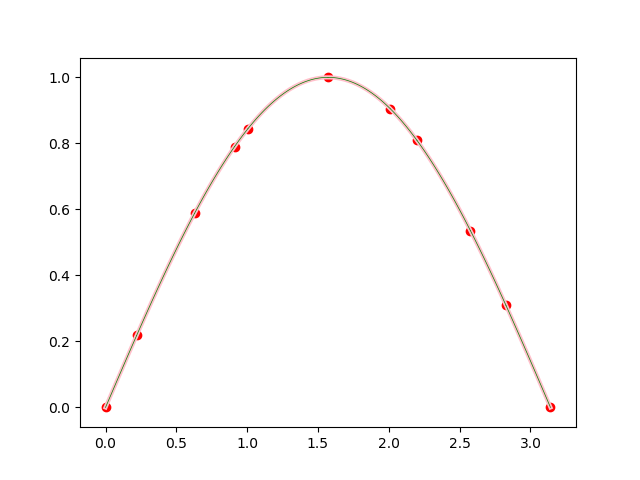
\includegraphics[width=10cm,height=9cm]{4-0_11.png}
  \caption{11个数据点,自然边界}
\end{figure}
\begin{figure}[H]
 \centering
  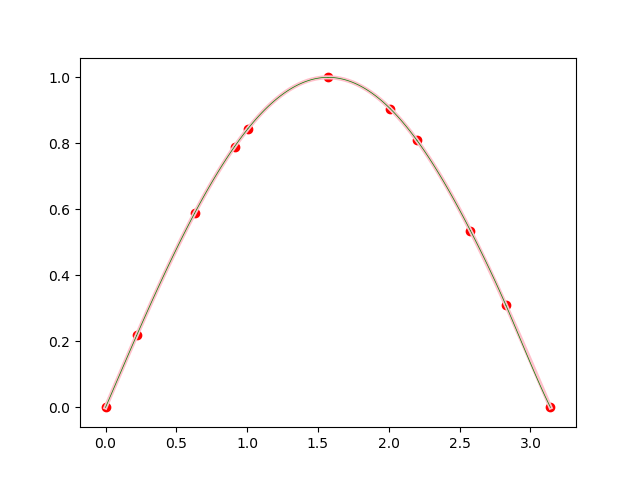
\includegraphics[width=10cm,height=9cm]{4-1_11.png}
  \caption{11个数据点,固定边界}
\end{figure}
\begin{figure}[H]
 \centering
  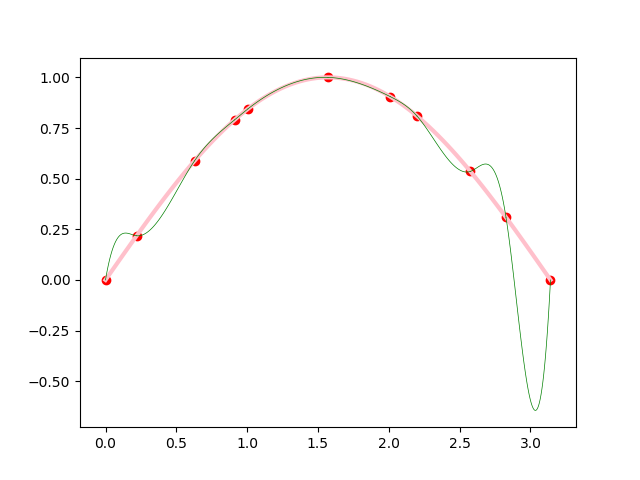
\includegraphics[width=10cm,height=9cm]{4-2_11.png}
  \caption{11个数据点,周期边界}
\end{figure}
\begin{figure}[H]
 \centering
  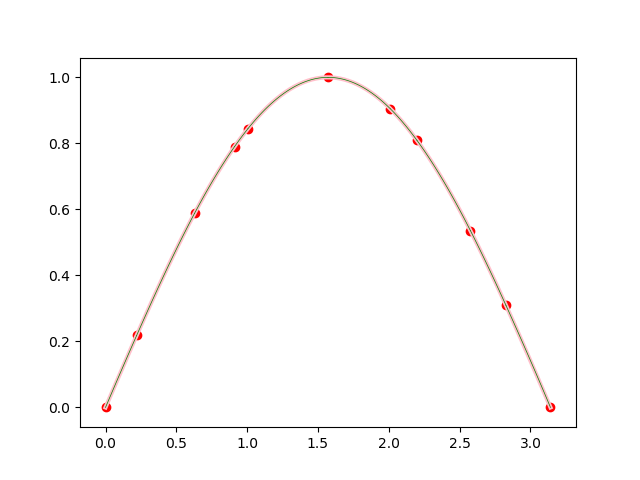
\includegraphics[width=10cm,height=9cm]{4-3_11.png}
  \caption{11个数据点,强制边界}
\end{figure}

\begin{figure}[H]
 \centering
  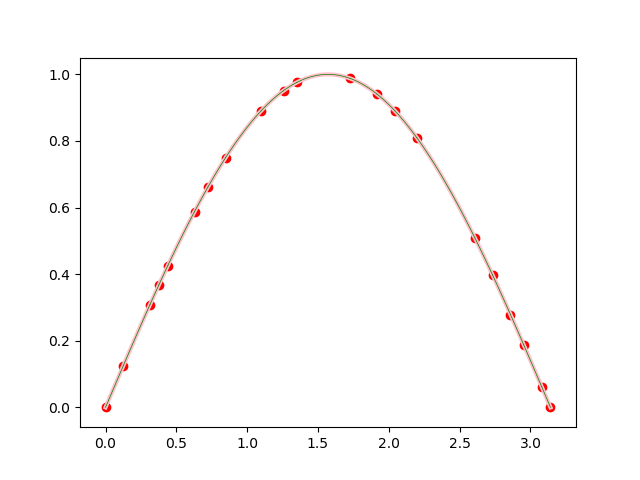
\includegraphics[width=10cm,height=9cm]{4-0_21.png}
  \caption{21个数据点,自然边界}
\end{figure}
\begin{figure}[H]
 \centering
  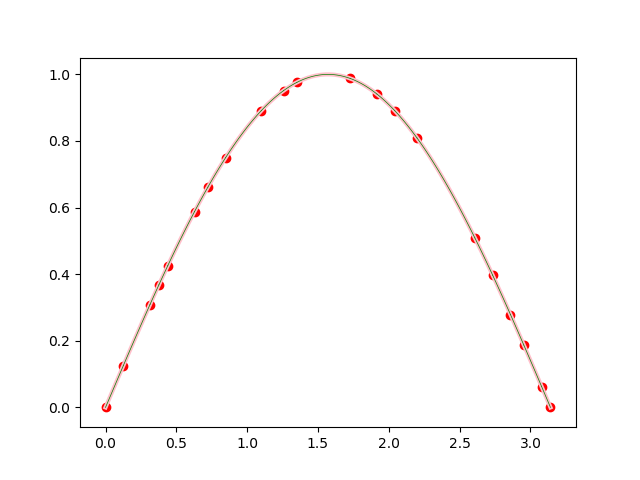
\includegraphics[width=10cm,height=9cm]{4-1_21.png}
  \caption{21个数据点,固定边界}
\end{figure}
\begin{figure}[H]
 \centering
  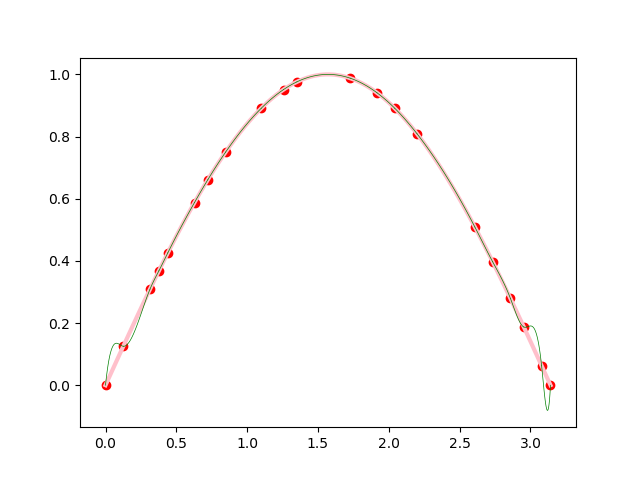
\includegraphics[width=10cm,height=9cm]{4-2_21.png}
  \caption{21个数据点,周期边界}
\end{figure}
\begin{figure}[H]
 \centering
  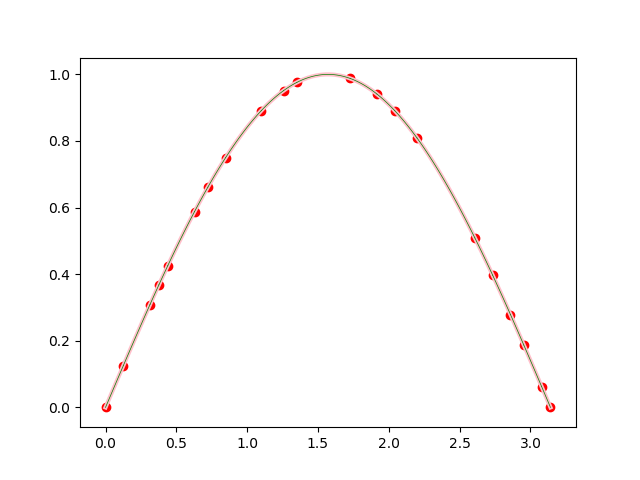
\includegraphics[width=10cm,height=9cm]{4-3_21.png}
  \caption{21个数据点,强制边界}
\end{figure}
\newpage

\subsection{作业推导}

~\\
~\\

给定在[a,b]上定义的函数f和一组节点$a=x_{0}<x_{1}<\cdots<x_{n}=b$ ,f的三次样条插值S是满足下列条件的函数:

a.S(x)在子区间$ [x_j,x_{j+1}(j=0,1,\cdots ,n-1) ]$上是三次多项式,记为$S_j(x)$

b.$S\left(x_{j}\right)=f\left(x_{j}\right)(j=0,1, \cdots, n)$

c.$S_{j+1}\left(x_{j+1}\right)=S_{j}\left(x_{j+1}\right)(j=0,1, \cdots, n-2)$

d.$S_{j+1}^{\prime}\left(x_{j+1}\right)=S_{j}^{\prime}\left(x_{j+1}\right)(j=0,1, \cdots, n-2)$

e.$S_{j+1}^{\prime \prime}\left(x_{j+1}\right)=S_{j}^{\prime \prime}\left(x_{j+1}\right)(j=0,1, \cdots, n-2)$

f.边界条件:

\quad (i) $S^{\prime \prime}\left(x_{0}\right)=\alpha_1$

\quad (ii)$S^{\prime \prime}\left(x_{0}\right)=\alpha_2$

\quad (iii)$
S^{\prime}\left(x_{0}\right)=\beta_1
$


\quad (iv)$
S^{\prime}\left(x_{0}\right)=\beta_2
$

为构造给定函数f的三次样条插值,把定义中的条件用到三次多项式:

$S_{j}(x)=a_{j}+b_{j}\left(x-x_{j}\right)+c_{j}\left(x-x_{j}\right)^{2}+d_{j}\left(x-x_{j}\right)^{3}, \quad j=0,1, \cdots, n-1$

因为

$S_{j}\left(x_{j}\right)=a_{j}=f\left(x_{j}\right)$

所以条件(c)可用于获得

$a_{j+1}=S_{j+1}\left(x_{j+1}\right)=S_{j}\left(x_{j+1}\right)=a_{j}+b_{j}\left(x_{j+1}-x_{j}\right)+c_{j}\left(x_{j+1}-x_{j}\right)^{2}+d_{j}\left(x_{j+1}-x_{j}\right)^{3}, \quad j=0,1, \cdots, n-2$

$h_{j}=x_{j+1}-x_{j}, \quad j=0,1, \cdots, n-1$

如果定义$a_n=f(x_n)$,则方程:

\begin{equation}
a_{j+1}=a_{j}+b_{j} h_{j}+c_{j} h_{j}^{2}+d_{j} h_{j}^{3}
\end{equation}

对$ j=0,1, \cdots, n-1$ 成立

定义$ b_n=S^{\prime}(x_n)$

$S_{j}^{\prime}(x)=b_{j}+2 c_{j}\left(x-x_{j}\right)+3 d_{j}\left(x-x_{j}\right)^{2}$

可得$$S_{j}^{\prime}\left(x_{j}\right)=b_{j}(j=0,1, \cdots, n-1)$$

应用条件(d)得到:

\begin{equation}
b_{j+1}=b_{j}+2 c_{j} h_{j}+3 d_{j} h_{j}^{2}, \quad j=0,1, \cdots, n-1
\end{equation}

定义$$
c_{n}=S^{\prime\prime}\left(x_{n}\right) / 2
$$

应用条件(e)得到:

\begin{equation}
c_{j+1}=c_{j}+3 d_{j} h_{j}
\end{equation}


在(5)中解出$d_j$并将解出的值带入(3)(4)中,得到新方程:

\begin{equation}
a_{j+1}=a_{j}+b_{j} h_{j}+\frac{h_{j}^{2}}{3}\left(2 c_{j}+c_{j+1}\right)
\end{equation}

\begin{equation}
b_{j+1}=b_{j}+h_{j}\left(c_{j}+c_{j+1}\right)
\end{equation}

解出$b_j$为:

\begin{equation}
b_{j}=\frac{1}{h_{j}}\left(a_{j+1}-a_{j}\right)-\frac{h_{j}}{3}\left(2 c_{j}+c_{j+1}\right)
\end{equation}

即下标减一得:

\begin{equation}
b_{j-1}=\frac{1}{h_{j-1}}\left(a_{j}-a_{j-1}\right)-\frac{h_{j-1}}{3}\left(2 c_{j-1}+c_{j}\right)
\end{equation}


从而得到线性方程组:

\begin{equation}
h_{j-1} c_{j-1}+2\left(h_{j-1}+h_{j}\right) c_{j}+h_{j} c_{j+1}=\frac{3}{h_{j}}\left(a_{j+1}-a_{j}\right)-\frac{3}{h_{j-1}}\left(a_{j}-a_{j-1}\right)
\end{equation}


对于以下四种边界,$$
a_{0}=f\left(x_{0}\right), a_{1}=f\left(x_{1}\right), \cdots, a_{n}=f\left(x_{n}\right)
$$
在解出$$ c_0 \cdots c_n$$后均有以下公式计算:


$$
\begin{array}{l}{b_{j}=\left(a_{j+1}-a_{j}\right) / h_{j}-h_{j}\left(c_{j+1}+2 c_{j}\right) / 3} \\ {d_{j}=\left(c_{j+1}-c_{j}\right) /\left(3 h_{j}\right)}\end{array}
$$


现在分析如何解出$$ c_0 \cdots c_n$$

1.对于自然边界:

$$S^{\prime\prime}(a)=0 $$ 

$$S^{\prime\prime}(b)=0 $$

得到$$ c_0=0,c_n=0$$

可得矢量方程$$ Ax=b$$


A为$$ (n+1)\times (n+1)$$矩阵


$$
A=\left[\begin{array}{lllllll}
{1} & {0} & {0} & {\cdots} & {\cdots} & {\cdots} & {\cdots} \\ 
{h_{0}} & {2\left(h_{0}+h_{1}\right)} & {h_{1}} & {\cdots} & {\cdots} & {\cdots} \\ 
{0} & {\cdots} & {h_{1} } & {2\left(h_{1}+h_{2}\right)} & {h} & {\cdots} & {\cdots} \\ 
{\vdots} & {\cdots} & {\cdots} & {\cdots} & {\cdots} & {\cdots} \\ 
{\vdots} & {} & {\cdots} & {\cdots} & {h_{n-2}} & { 2(h_{n-2}+h_{n-1})} & {h_{n-1}} \\ 
{0} & {\cdots} & {\cdots} & {\cdots}  & {0} & {0} & {1}
\end{array}\right]
$$

b和x为向量:


$$
b=\left[\begin{array}{c}{0} \\ {\frac{3}{h_{1}}\left(a_{2}-a_{1}\right)-\frac{3}{h_{0}}\left(a_{1}-a_{0}\right)} \\ {\vdots} \\ {\frac{3}{h_{n-1}}\left(a_{n}-a_{n-1}\right)-\frac{3}{h_{n-2}}\left(a_{n-1}-a_{n-2}\right)} \\ {0}\end{array}\right]
$$


$$
\boldsymbol{x}=\left[\begin{array}{c}{c_{0}} \\ {c_{1}} \\ {\vdots} \\ {c_{n}}\end{array}\right]
$$

2.固定边界

$$ S^{\prime}(x_0)=f^{\prime}(x_0)$$

$$ S^{\prime}(x_n)=f^{\prime}(x_n)$$

$$
b_{0}=f^{\prime}(x_0)=\frac{1}{h_{0}}\left(a_{1}-a_{0}\right)-\frac{h_{0}}{3}\left(2 c_{0}+c_{1}\right)
$$

$$
b_{n-1}=f^{\prime}(x_{n-1})=\frac{1}{h_{n-1}}\left(a_{n}-a_{n-1}\right)-\frac{h_{n-1}}{3}\left(2 c_{n-1}+c_{n}\right)
$$
可得矢量方程$$ Ax=b$$


A为$$ (n+1)\times (n+1)$$矩阵


$$
A=\left[\begin{array}{lllllll}
{2h_0} & {h_0} & {0} & {\cdots} & {\cdots} & {\cdots} & {\cdots} \\ 
{h_{0}} & {2\left(h_{0}+h_{1}\right)} & {h_{1}} & {\cdots} & {\cdots} & {\cdots} \\ 
{0} & {\cdots} & {h_{1} } & {2\left(h_{1}+h_{2}\right)} & {h} & {\cdots} & {\cdots} \\ 
{\vdots} & {\cdots} & {\cdots} & {\cdots} & {\cdots} & {\cdots} \\ 
{\vdots} & {} & {\cdots} & {\cdots} & {h_{n-2}} & { 2(h_{n-2}+h_{n-1})} & {h_{n-1}} \\ 
{0} & {\cdots} & {\cdots} & {\cdots}  & {0} & {h_{n-1}} & {2h_{n-1}}
\end{array}\right]
$$

b和x为向量:


$$
b=\left[\begin{array}{c}{\frac{3}{h_{1}}\left(a_{2}-a_{1}\right)-{3}{f^{\prime}(a)}} \\ {\frac{3}{h_{1}}\left(a_{2}-a_{1}\right)-\frac{3}{h_{0}}\left(a_{1}-a_{0}\right)} \\ {\vdots} \\ {\frac{3}{h_{n-1}}\left(a_{n}-a_{n-1}\right)-\frac{3}{h_{n-2}}\left(a_{n-1}-a_{n-2}\right)} \\ {3}{f^{\prime}(b)}-\frac{3}{h_{n-1}}(a_n-a_{n-1})\end{array}\right]
$$


$$
\boldsymbol{x}=\left[\begin{array}{c}{c_{0}} \\ {c_{1}} \\ {\vdots} \\ {c_{n}}\end{array}\right]
$$




 3.周期边界
$$b_0=b_n
$$

$$
c_0=c_n
$$

可得矢量方程$$ Ax=b$$


A为$$ (n+1)\times (n+1)$$矩阵


$$
A=\left[\begin{array}{lllllll}
{\frac{2}{3}h_0} & {\frac{1}{3}h_0} & {0} & {\cdots} & {\cdots} & {-\frac{2}{3}h_{n-1}} & {-\frac{1}{3}h_{n-1}} \\ 
{h_{0}} & {2\left(h_{0}+h_{1}\right)} & {h_{1}} & {\cdots} & {\cdots} & {\cdots} \\ 
{0} & {\cdots} & {h_{1} } & {2\left(h_{1}+h_{2}\right)} & {h} & {\cdots} & {\cdots} \\ 
{\vdots} & {\cdots} & {\cdots} & {\cdots} & {\cdots} & {\cdots} \\ 
{\vdots} & {} & {\cdots} & {\cdots} & {h_{n-2}} & { 2(h_{n-2}+h_{n-1})} & {h_{n-1}} \\ 
{1} & {\cdots} & {\cdots} & {\cdots}  & {0} & {0} & {-1}
\end{array}\right]
$$

b和x为向量:


$$
b=\left[\begin{array}{c}{ \frac{1}{h_0}(a_1-a_0) - \frac{1}{h_{n-1}}(a_{n}-a_{n-1})} \\ {\frac{3}{h_{1}}\left(a_{2}-a_{1}\right)-\frac{3}{h_{0}}\left(a_{1}-a_{0}\right)} \\ {\vdots} \\ {\frac{3}{h_{n-1}}\left(a_{n}-a_{n-1}\right)-\frac{3}{h_{n-2}}\left(a_{n-1}-a_{n-2}\right)} \\ {0}\end{array}\right]
$$


$$
\boldsymbol{x}=\left[\begin{array}{c}{c_{0}} \\ {c_{1}} \\ {\vdots} \\ {c_{n}}\end{array}\right]
$$


4.强制第一个子区间和第二个子区间样条多项式的三阶导数相同,倒数第二个子区间和最后一个子区间的三次样条函数的三阶导数相等


可得矢量方程$$ Ax=b$$


A为$$ (n+1)\times (n+1)$$矩阵


$$
A=\left[\begin{array}{lllllll}
{1} & {-1} & {\cdots} & {\cdots} & {\cdots} & {\cdots} \\ 
{h_{0}} & {2\left(h_{0}+h_{1}\right)} & {h_{1}} & {\cdots} & {\cdots} & {\cdots} \\ 
{0} & {\cdots} & {h_{1} } & {2\left(h_{1}+h_{2}\right)} & {h} & {\cdots} & {\cdots} \\ 
{\vdots} & {\cdots} & {\cdots} & {\cdots} & {\cdots} & {\cdots} \\ 
{\vdots} & {} & {\cdots} & {\cdots} & {h_{n-2}} & { 2(h_{n-2}+h_{n-1})} & {h_{n-1}} \\ 
{0} & {\cdots} & {\cdots} & {\cdots}  & {0} & {1} & {-1}
\end{array}\right]
$$

b和x为向量:


$$
b=\left[\begin{array}{c}{ 0} \\ {\frac{3}{h_{1}}\left(a_{2}-a_{1}\right)-\frac{3}{h_{0}}\left(a_{1}-a_{0}\right)} \\ {\vdots} \\ {\frac{3}{h_{n-1}}\left(a_{n}-a_{n-1}\right)-\frac{3}{h_{n-2}}\left(a_{n-1}-a_{n-2}\right)} \\ {0}\end{array}\right]
$$


$$
\boldsymbol{x}=\left[\begin{array}{c}{c_{0}} \\ {c_{1}} \\ {\vdots} \\ {c_{n}}\end{array}\right]
$$


\newpage





\section{第四章数值微分与数值积分}
\subsection{problem 1}

1.编制复合梯形公式、Simpson公式的计算程序。

2.取 h=0.01,分别利用复合梯形、Simpson公式计算定积分:

$ I(f)=\frac{1}{\sqrt{2 \pi}} \int_{0}^{1} \exp ^{-\frac{x^{2}}{2}} \mathrm{d} x $

3.取计算精度为$ 10 ^ {-4} $,则h=?,n=?


python实现代码如下:
\begin{lstlisting}
	import math

	from scipy import integrate


	def f(x):
	    t = 1 / pow(2 * math.pi, 0.5)
	    return t * pow(math.e, (-0.5 * x * x))


	truevalue, e = integrate.quad(f, 0, 1)

	print(truevalue)

	n1 = 1000
	n2 = 1000


	# n % 2 ==0
	def Simpson(a=0, b=1, n=n1):
	    h = (b - a) / n
	    fx = []
	    for i in range(n + 1):
	        fx.append(f(a + h * i))
	    res = 0
	    for i in range(n + 1):
	        if i == 0:
	            res += fx[i]
	            continue
	        if i == n:
	            res += fx[i]
	            continue
	        if i % 2 == 0:
	            res += 2 * fx[i]
	        if i % 2 == 1:
	            res += 4 * fx[i]
	    res = res * h / 3
	    error = truevalue - res
	    return res, error


	def Compsite(a=0, b=1, n=n2):
	    h = (b - a) / n
	    fx = []
	    for i in range(n + 1):
	        fx.append(f(a + h * i))
	    res = 0
	    for i in range(n + 1):
	        if i == 0:
	            res += fx[i]
	            continue
	        if i == n:
	            res += fx[i]
	            continue
	        res += 2 * fx[i]
	    res = res * h / 2
	    error = truevalue - res
	    return res, error


	print('SIMPSON', Simpson())
	print('Compsite', Compsite())

	error0 = 1e-4


	def find1(a=0, b=1, error=error0):
	    res = 0
	    for i in range(10, 1000):
	        v, e = Simpson(a=a, b=b, n=i)
	        if abs(e) < error:
	            res = i
	            break
	    h = (b - a) / res
	    n = res
	    return h, n


	def find2(a=0, b=1, error=error0):
	    res = 0
	    for i in range(10, 1000):
	        v, e = Compsite(a=a, b=b, n=i)
	        if abs(e) < error:
	            res = i
	            break
	    h = (b - a) / res
	    n = res
	    return h, n


	print(find1())
	print(find2())

\end{lstlisting}

使用scipy的integrate模块的到精确解为0.341344746068543

在同样迭代1000轮的情况下


使用复合梯形公式计算结果为:0.341344746068546,误差为$ -2.9976021664879227 \times 10^{-15} $

使用Simpson公式计算结果为:0.3413447259043159,误差为$ 2.01642270658553 \times 10^{-8} $

对于复合梯形公式,取计算精度为$ 10 ^ {-4} $,则h=0.1 ,n=10

对于Simpson公式,取计算精度为$ 10 ^ {-4} $,则h=0.06666666666666667 ,n=15


由此见得在同样迭代轮次的情况下,复合梯形公式计算更高。







\newpage
\subsection{作业推导}
~\\
1(i).推导复合梯形公式及其误差估计

证明:

在每个子区间$$[x_{k-1},x_k]$$上应用梯形公式


$$\int_{a}^{b} = \Sigma_{k=1}^{M} \int_{x_{k-1}}^{x_k} \approx \Sigma_{k=1}^{M} \frac{h}{2} ((f(x_{k-1}))+(f(x_k))) $$


由于$\frac{h}{2}$ 为常数,由加法分配律可得


$$
T(f,h)= \frac{h}{2} \Sigma_{k=1}^{M}  ((f(x_{k-1}))+(f(x_k)))
$$

或

$$
T(f,h)=\frac{h}{2} (f(a)+f(b)) + h \Sigma_{k=1}^{M-1} x_k
$$

它们是区间[a,b]上f(x)积分的逼近,记为:

$$
\int_{b}^{a} f(x) dx \approx T(f,h)$$




$$
E_T (f,h)=a_1h^2+a_2h^4+a_3h^6\cdots
$$






~\\



1(ii).推导基于误差控制的逐次半积分梯形公式及其误差估计


运用梯形公式:

$$\int_{a}^{b} f(x) dx =T(f,h)+E_T (f,h)$$


$$
E_T (f,h)=a_1h^2+a_2h^4+a_3h^6\cdots
$$


$$
\int_{a}^{b} f(x) dx=T(f,h)+a_1h^2+a_2h^4+a_3h^6\cdots
$$

$$
4\int_{a}^{b} f(x) dx=4T(f,h)+4a_1h^2+4a_2h^4+4a_3h^6\cdots
$$

$$
\int_{a}^{b} f(x) dx=T(f,2h)+a_14h^2+a_216h^4+a_364h^6\cdots
$$


下减上得

$$
\int_{a}^{b} f(x) dx=\frac{4T(f,h)-T(f,2h)}{3}+b_1h^4+b_2h^6\cdots
$$

误差降低为 $O(h^4)$


~\\
2.let $ h= \frac{b-a}{3} , x_0=a,x_1=a+h,x_2=b$.Find the degree of percision of the quadrature formula


$$\int_{a}^{b} f(x) dx=\frac{9}{4}hf(x_1)+\frac{3}{4}hf(x_2)$$


解:

$$
\delta =b-a
$$

$$
T(f,b-a)=\frac{1}{2} (b-a) (f(x_0)+f(x_2)) 
= \frac{1}{2} \delta (f(x_0)+f(x_2)) 
$$


$$
T(f,\frac{b-a}{3})-=\frac{1}{2} \frac{1}{3}(b-a) (f(x_0)+f(x_1))  +\frac{1}{2} \frac{2}{3}(b-a) (f(x_1)+f(x_2))
$$

$$
= \frac{1}{6} \delta f(x_0)+ \frac{1}{2} \delta f(x_1) + \frac{1}{3} \delta f(x_2)
$$

3倍的下减上得:


$$
\int_{a}^{b} f(x) dx \approx \frac{3T(f,\frac{b-a}{3})-T(f,b-a)}{2}
$$

$$
E_T (f,3h)=\frac{(3h)f^{(2)}(c_1)(3h)^2}{12}
$$

$$
E_T (f,h)=\frac{(h)f^{(2)}(c_2)(h)^2}{12}+\frac{(2h)f^{(2)}(c_3)(2h)^2}{12}
$$

$$
Error=3E_T (f,h)-E_T (f,3h)=O(h^4)
$$



\newpage


\section{第五章常微分方程数值解}

\subsection{problem 1}
求$ y^{\prime}=1+y^{2}, y(0)=0$ 的数值解(分别用欧拉显格式、梯形预估修正格式、4阶龙格库塔格式,并与解析解比较三种格式的收敛性)


python实现代码如下:
\begin{lstlisting}	

	import numpy as np
	import matplotlib.pyplot as plt
	import math

	N = 10


	def f(t, w):
	    return 1 + w * w


	def pt(res, color):
	    plt.scatter(np.array(res).T[0], np.array(res).T[1], color=color)


	def inplot():
	    x = np.linspace(0, np.pi / 2.2, 100, endpoint=True)
	    y = np.tan(x)
	    plt.plot(x, y, color='pink', linewidth=3)


	def Euler(a=0, b=math.pi / 2.2, n=N, alpha=0):
	    h = (b - a) / n
	    t = a
	    w = alpha
	    res = [[t, w]]
	    for i in range(1, n):
	        w += h * f(t, w)
	        t += h
	        res.append([t, w])

	    return res


	def improvedEuler(a=0, b=math.pi / 2.2, n=N, alpha=0):
	    h = (b - a) / n
	    t = a
	    w = alpha
	    res = [[t, w]]
	    for i in range(1, n):
	        t1 = w + h * f(t, w)
	        w += h / 2 * (f(t, w) + f(t + h, t1))
	        t += h
	        res.append([t, w])
	    return res


	def RungeKutta(a=0, b=math.pi / 2.2, n=N, alpha=0):
	    h = (b - a) / n
	    t = a
	    w = alpha
	    res = [[t, w]]
	    for i in range(1, n):
	        k1 = h * f(t, w)
	        k2 = h * f(t + h / 2, w + k1 / 2)
	        k3 = h * f(t + h / 2, w + k2 / 2)
	        k4 = h * f(t + h / 2, w + k3)
	        w += (k1 + 2 * k2 + 2 * k3 + k4) / 6
	        t += h
	        res.append([t, w])
	    return res


	res1 = Euler()
	pt(res1, 'green')

	res2 = improvedEuler()
	pt(res2, 'red')

	res3 = RungeKutta()
	pt(res3, 'blue')

	inplot()

	plt.show()

\end{lstlisting}
\begin{figure}[H]
 \centering0
  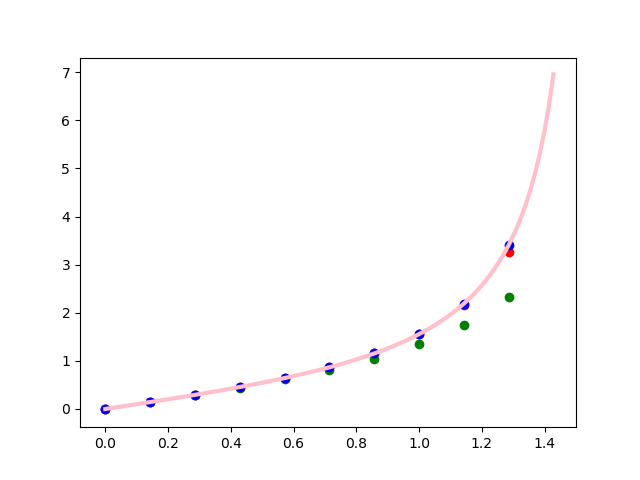
\includegraphics[width=10cm,height=9cm]{6-0.png}
  \caption{green:Euler,red:improvedEuler,blue:RungeKutta}
\end{figure}







由收敛图像可见,欧拉显格式、梯形预估修正格式、4阶龙格库塔格式,三者收敛速率逐个下降。


\subsection{problem 2}

用龙格库塔4阶方法求解描述振荡器的经典的van der Plo 微分方程:

$\left\{\begin{array}{l}{\frac{\mathrm{d}^{2} y}{\mathrm{d} t^{2}}-\mu\left(1-y^{2}\right) \frac{\mathrm{d} y}{\mathrm{d} t}+y=0} \\ {y(0)=1, y^{\prime}(0)=0}\end{array}\right.$

分别取$ \mu =0.01 ,0.1 ,1$ ,作图比较计算结果

python实现代码如下:

\begin{lstlisting}	
	import numpy as np
	import matplotlib.pyplot as plt
	import math

	N = 1000
	mu = 0.01


	def f1(t, w1, w2):
	    return w2


	def f2(t, w1, w2):
	    return mu * (1 - w1 * w1) * w2 - w1


	def pt(res):
	    plt.plot(np.array(res).T[0], np.array(res).T[1])
	    plt.show()
	    plt.plot(np.array(res).T[0], np.array(res).T[2])
	    plt.show()

	def RungeKutta2(a=0, b=10, n=N, alpha=1 , alpha1=0):
	    h = (b - a) / n
	    t = a
	    w1 = alpha
	    w2 = alpha1
	    res=[[t,w1,w2]]
	    for i in range(N):
	        k11=h*f1(t,w1,w2)
	        k12=h*f2(t,w1,w2)
	        k21=h*f1(t+h/2,w1+k11/2,w2+k12/2)
	        k22=h*f2(t+h/2,w1+k11/2,w2+k12/2)
	        k31=h*f1(t+h/2,w1+k21/2,w2+k22/2)
	        k32=h*f2(t+h/2,w1+k21/2,w2+k22/2)
	        k41=h*f1(t+h/2,w1+k31/2,w2+k32/2)
	        k42=h*f2(t+h/2,w1+k31/2,w2+k32/2)
	        w1+=(k11+2*k21+2*k31+k41)/6
	        w2+=(k12+2*k22+2*k32+k42)/6
	        t+=h
	        res.append([t,w1,w2])
	    return res


	res=RungeKutta2()
	pt(res)
\end{lstlisting}
$ \mu =0.01 $时:

\begin{figure}[H]
 \centering
  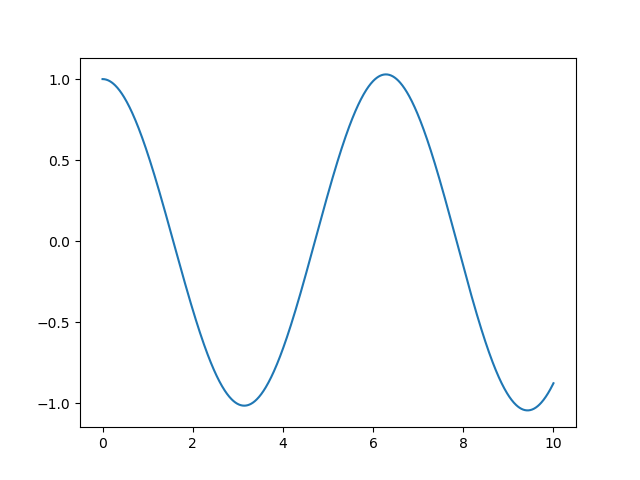
\includegraphics[width=10cm,height=9cm]{6-001-01.png}
  \caption{y-t}
\end{figure}

\begin{figure}[H]
 \centering
  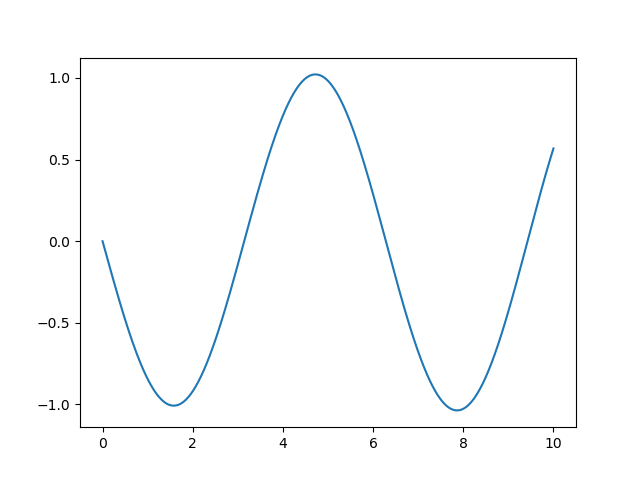
\includegraphics[width=10cm,height=9cm]{6-001-02.png}
  \caption{y'-t}
\end{figure}


$ \mu =0.1 $时:

\begin{figure}[H]
 \centering
  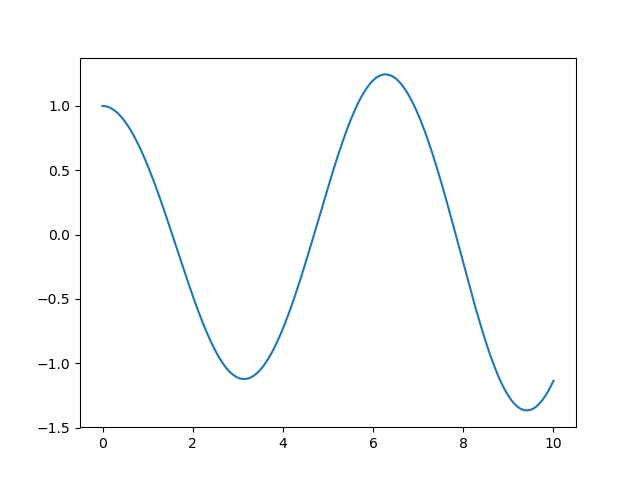
\includegraphics[width=10cm,height=9cm]{6-01-01.png}
  \caption{y-t}
\end{figure}

\begin{figure}[H]
 \centering
  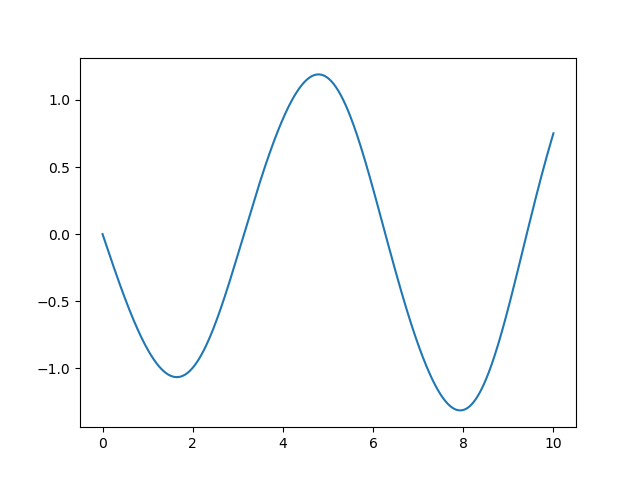
\includegraphics[width=10cm,height=9cm]{6-01-02.png}
  \caption{y'-t}
\end{figure}


$ \mu =1 $时:

\begin{figure}[H]
 \centering
  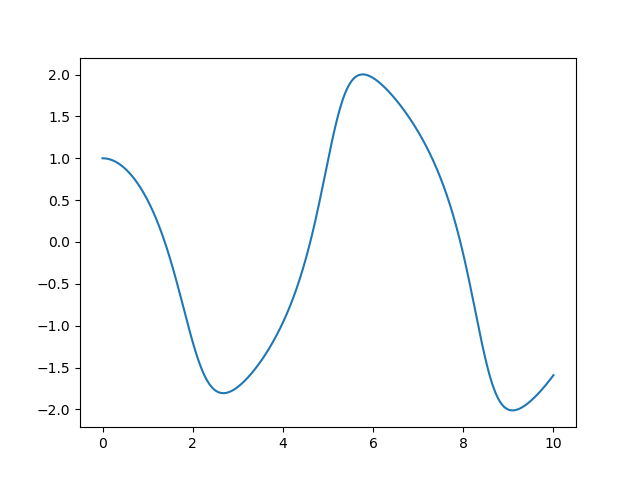
\includegraphics[width=10cm,height=9cm]{6-1-01.png}
  \caption{y-t}
\end{figure}

\begin{figure}[H]
 \centering
  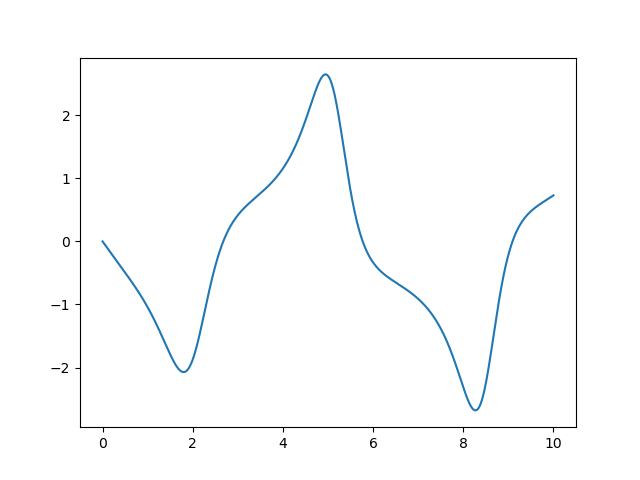
\includegraphics[width=10cm,height=9cm]{6-1-02.png}
  \caption{y'-t}
\end{figure}

\newpage

\section{第八章曲线拟合与函数逼近}


已知观测数据:

\begin{table}[H]
\centering
\caption{x-f(X)}
\begin{tabular}{|l|l|l|l|l|l|}
\hline

x & -2 & -1 & 0 & 1 & 2 \\ \hline
f(x) & 0  & 1 & 2 & 1 & 0 \\ \hline

\end{tabular}
\end{table}

求一个二次多项式拟合数据,写出最小二乘拟合模型,给出正则方程组及其解



python实现代码如下:
\begin{lstlisting}	
	import numpy as np

	x_array = np.array([-2, -1, 0, 1, 2])
	y_array = np.array([0,1,2,1,0])
	n = 2
	m = len(x_array)  

	A = np.ones(m).reshape((m, 1))
	for i in range(n):
	    A = np.hstack([A, (x_array ** (i + 1)).reshape((m, 1))])

	from numpy.linalg import solve
	alpha=np.dot(A.T, A)
	belta= np.dot(A.T, y_array.T)
	X = solve(alpha,belta)
	print(X)
	print(alpha)
	print(belta)
	import matplotlib.pyplot as plt

	x = np.linspace(-3, 3, 100, endpoint=True)
	y = X[2]*x*x+X[1]*x+X[0]
	plt.plot(x, y,color='pink',linewidth=1)
	plt.scatter(x_array,y_array)
	plt.show()


\end{lstlisting}

\begin{figure}[H]
 \centering
  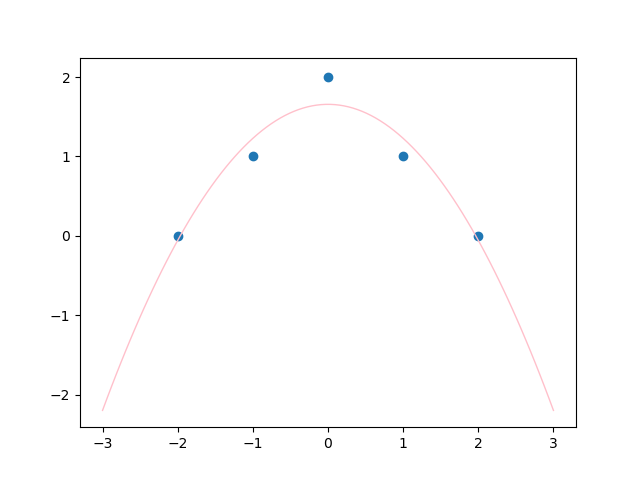
\includegraphics[width=10cm,height=9cm]{8.png}
  \caption{拟合图像}
\end{figure}

拟合方程为$ y=1.65714286-0.42857143x^2$

正则方程组如下:

$5X_0+0+10X_2=4 $

$0+10X_1+0=0 $

$10X_0+0+34X_2=2 $

方程的解为:$X_0=1.65714286 , X_1=0 , X_2=-0.42857143$
\newpage

\section{第九章特征值与特征向量}
\subsection{problem 1}
已知矩阵:

$\mathbf{A}=\left[\begin{array}{ccc}{4} & {-1} & {1} \\ {-1} & {3} & {-2} \\ {1} & {-2} & {3}\end{array}\right]$

是一个对称矩阵,且其特征值为$ \lambda_1 =6, \lambda_2 =3, \lambda_3 =1 $,

分别利用幂法、对称幂法、反幂法求其最大特征值和特征向量。

初始向量$ \mathbf{x}^{(0)}=(1\quad 1 \quad1)^{T} $
python实现代码如下:
\begin{lstlisting}
	import numpy as np

	A0 = [
	    [4, -1, 1],
	    [-1, 3, -2],
	    [1, -2, 3]
	]
	A = np.array(A0)




	def findmax(x):
	    t = np.abs(x).tolist()
	    xmax = np.max(t)
	    res = 0
	    for i in range(len(t)):
	        if t[i] == xmax:
	            res = i
	            break
	    return xmax, res


	def f1(N=1000000, TOL=1e-18):
	    xr=[]
	    x = [1, 1, 1]
	    X = np.array(x).T
	    k = 1
	    xmax, p = findmax(X)
	    X = X / xmax
	    while k < N:
	        k += 1
	        y = np.matmul(A, X)
	        ymax, yp = findmax(y)
	        mu = ymax
	        xr.append(mu)
	        if ymax == 0:
	            print(X)
	            print('please reselect x')
	            break
	        err, no = findmax(X - (y.T) / ymax)
	        X = y.T / ymax

	        if err < TOL:
	            xm, xp = findmax(X)
	            return mu, X/xm, k,xr
	            break


	print(f1())


	def two(X):
	    sum = 0
	    for i in X:
	        sum += i * i
	    sum = pow(sum, 0.5)
	    return sum


	def f2(N=1000000, TOL=1e-18):
	    x = [1, 1, 1]
	    xr = []
	    X = np.array(x).T
	    X = X / two(X)
	    k = 1
	    while k <= N:
	        k += 1
	        y = np.matmul(A, X)
	        mu = np.matmul(X.T, y)
	        xr.append(mu)
	        if two(y) == 0:
	            print('Eig', X)
	            print('reselect')
	        ERR = two(X - y / two(y))
	        X = y / two(y)
	        if ERR < TOL:
	            xm,xp=findmax(X)
	            return mu, X/xm, k,xr


	print(f2())


	def cal(A, B):
	    x = np.linalg.solve(A, B)
	    return x.T


	def calq(X):
	    q = np.matmul(np.matmul(X.T, A), X) / np.matmul(X.T, X)
	    return q


	def f3(N=100000, TOL=1e-18):
	    x = [1, -0.1, 0.2]
	    xr=[]
	    X = np.array(x).T
	    k = 1
	    q = calq(X)
	    xr.append(q)
	    xmax, xp = findmax(X)
	    X = X / xmax

	    while k <= N:
	        k += 1
	        I = np.eye(len(A))
	        q = calq(X)
	        xr.append(q)
	        try:
	            y = np.array(cal(A - q * I, X)).T
	        except:
	            ymax, yp = findmax(y)
	            return q, y/ ymax, k,xr
	        else:
	            ymax, yp = findmax(y)
	            mu = ymax
	            ERR, no = findmax(X - (y / ymax))
	            X = y / ymax

	            if ERR < TOL:
	                mu = (1 / mu) + q
	                xm, xp = findmax(X)
	                return mu, X/xm, k,xr


	print(f3())
	
\end{lstlisting}

1.幂法

设置初始向量$ \mathbf{x}^{(0)}=(1\quad 1 \quad1)^{T} $。

用如下递归公式生成序列

$$
Y_k=AX_k
$$


$$
X_{k+1}=\frac{1}{C_{k+1}} Y_k
$$

其中$C_{k+1}$是$Y_k$绝对值最大的分量。序列{$X_k$}和序列{$C_k$}将分别收敛到最大特征值$\lambda$和对应的特征向量V。

我们可以证明$X_k$收敛到V的速度是由项$ (\frac{\lambda_2}{\lambda_1})^k$决定,所以收敛速度为线性。

2.反幂法

与幂法不同,我们在求解Y的时候,使用的不是

$$
Y_k=AX_k
$$

而是 

$$
Y_{k}=(A-\alpha I)^{-1} X_{k}
$$

最终我们得到的特征值是


$$
\lambda_{\mathrm{j}}=\frac{1}{\mu_{1}}+\alpha
$$

也就是说,我们得到的特征值是最接近$\alpha$的特征值,随意为了求解对应的特征值,我们必须
选择一个相近的初值.

3.对称幂法

对称幂法使用的基本原理是

$$
\begin{array}{c}{\lim _{\mathbf{k} \rightarrow \infty} \frac{x_{k}^{T} A x_{k}}{x_{k}^{T} x_{k}}=\lambda_{1}} \\ {\lim _{\mathbf{k} \rightarrow \infty} \frac{x_{k}}{\left\|x_{k}\right\|_{2}}=\frac{V^{(1)}}{|| V^{(1)}||_{2}}}\end{array}
$$


它的A的收敛速度是$$
\mathrm{O}\left(\left|\frac{\lambda_{1}}{\lambda_{2}}\right|^{2 \mathrm{m}}\right)
$$序列的收敛速度$$
\left\{\mu^{(\mathrm{m})}\right\}_{m=1}^{\infty}
$$仍然是线性的。





实验结果:

1.幂法获得最大特征值为6,特征向量为$ (1\quad -1 \quad1)^{T}$,迭代次数为57,误差为$ 10^{-18}$

2.对称幂法获得最大特征值为6,特征向量为$ (1\quad -1 \quad1)^{T}$,迭代次数为56,误差为$ 10^{-18}$


3.反幂法获得最大特征值为6,特征向量为$ (1\quad -1 \quad1)^{T}$,迭代次数为8,误差为$ 10^{-18}$







\subsection{problem 2}


对于数据:

$\mathbf{A}=\left[\begin{array}{ccc}{1} & {-1} & {1.0} \\ 
									{1} & {-0.5} & {0.25} \\ 
									{1} & {0.0} & {0.0} \\ 
									{1} & {0.5} & {0.25} \\
									 {1} & {1.0} & {1.0}\end{array}\right]$


$ \mathbf{b}=\left[\begin{array}{l}{1.0} \\ {0.5} \\ {0.0} \\ {0.5} \\ {2.0}\end{array}\right]$

进行Household变换,输出$H_1,H_2,H_3$

python实现代码如下:
\begin{lstlisting}	
	import numpy as np





	a = [
	    [1, -1, 1],
	    [1, -0.5, 0.25],
	    [1, 0, 0],
	    [1, 0.5, 0.25],
	    [1, 1, 1]
	]
	b = [1, 0.5, 0, 0.5, 2]
	I = np.eye(5)

	A = np.array(a).T
	B = np.array(b).T


	def vvt(v):
	    res = np.zeros((len(v),len(v)))
	    for i in range(len(v)):
	        for j in range(len(v)):
	            res[i][j] = v[i] * v[j]
	    return res



	def vtv(v):
	    sum = 0
	    for i in range(len(v)):
	            sum  += v[i] * v[i]
	    return sum

	def vvt1(v):
	    return vvt(v)/vtv(v)


	def H(v):
	    I=np.eye(len(v))
	    H=I-2*vvt1(v)
	    return H

	def HA(v,A):
	    return np.matmul(H(v),A.T)

	def HB(H,B):
	    return np.matmul(H,B)


	def createv(A,A0,k,j):
	    s1=0
	    for i in range(k,len(A0[k])):
	        s1+=pow(A0[k][i],2)
	    s1=pow(s1,0.5)
	    res=[]
	    for fk in A[k]:
	        res.append(fk)
	    for i in range(j):
	        res[i]=0
	    if A[k][j]>0:
	        res[j]+=s1
	    else:
	        res[j]-=s1
	    return res
	v1=createv(A,A,0,0)
	H1=H(v1)
	A1=np.array(HA(v1,A))
	print(A1)
	A1=A1.T
	v2=createv(A1,A,1,1)
	H2=H(v2)
	A2=np.array(HA(v2,A1))
	print(A2)
	A2=A2.T
	v3=createv(A2,A,2,2)
	H3=H(v3)
	A3=HA(v3,A2)
	print(A3)


	B1=HB(H1,B)
	print(B1)
	B2=HB(H2,B1)
	print(B2)
	B3=HB(H3,B2)
	print(B3)
\end{lstlisting}
实验结果:
$\mathbf{H_1}=\left[\begin{array}{cccccc}
									{-0.4472}&{-0.4472}&{-0.4472}&{-0.4472}&{-0.4472}\\
{-0.4472}&{0.86180}&{-0.1381}&{-0.1381}&{-0.1381}\\
{-0.4472}&{-0.1381}&{0.86180}&{-0.1381}&{-0.1381}\\
{-0.4472}&{-0.1381}&{-0.1381}&{0.86180}&{-0.1381}\\
{-0.4472}&{-0.1381}&{-0.1381}&{-0.1381}&{0.86180}
									 \end{array}\right]$


$\mathbf{H_2}=\left[\begin{array}{cccccc}
									{1.0}&{0.0}&{0.0}&{0.0}&{0.0}\\
{0.0}&{0.10278}&{0.19583}&{0.51271}&{0.82958}\\
{0.0}&{0.19583}&{0.95725}&{-0.1119}&{-0.1810}\\
{0.0}&{0.51271}&{-0.1119}&{0.70701}&{-0.4740}\\
{0.0}&{0.82958}&{-0.1810}&{-0.4740}&{0.23294}
									 \end{array}\right]$



$\mathbf{H_3}=\left[\begin{array}{cccccc}
									{1.0}&{0.0}&{0.0}&{0.0}&{0.0}\\
{0.0}&{1.0}&{0.0}&{0.0}&{0.0}\\
{0.0}&{0.0}&{-0.7988}&{-0.5989}&{0.05660}\\
{0.0}&{0.0}&{-0.5989}&{0.80059}&{0.01884}\\
{0.0}&{0.0}&{0.05660}&{0.01884}&{0.99821}
									 \end{array}\right]$


用以上$H_1,H_2,H_3$得出的$H_1A,H_1b,H_2H_1A,H_2H_1b,H_3H_2H_1A,H_3H_2H_1b$如下:

$\mathbf{H_1A}=\left[\begin{array}{cccccc}
									{-2.2360}&{5.55111}&{5.55111}&{2.77555}&{0.0}\\
{-5.5511}&{-0.1909}&{0.30901}&{0.80901}&{1.30901}\\
{-1.1180}&{-0.4045}&{-0.6545}&{-0.4045}&{0.34549}
									 \end{array}\right]$

$\mathbf{H_1b}=\left[\begin{array}{cccccc}
									{-1.7888}\\
{-0.3618}\\
{-0.8618}\\
{-0.3618}\\
{1.13819}
									 \end{array}\right]$



$\mathbf{H_2H_1A}=\left[\begin{array}{cccccc}
									{-2.2360}&{3.08077}&{6.09032}&{4.18723}&{2.28414}\\
{-5.5511}&{1.54161}&{-0.0691}&{-0.1810}&{-0.2929}\\
{-1.1180}&{-0.0905}&{-0.7230}&{-0.5839}&{0.05518}
									 \end{array}\right]$


$\mathbf{H_2H_1b}=\left[\begin{array}{cccccc}
									{-1.7888}\\
{0.55276}\\
{-1.0614}\\
{-0.8844}\\
{0.29256}
									 \end{array}\right]$


$\mathbf{H_3H_2H_1A}=\left[\begin{array}{cccccc}
									{-2.2360}&{-5.5511}&{-1.1180}\\
{3.08077}&{1.54161}&{-0.0905}\\
{-7.2435}&{0.14711}&{0.93041}\\
{-2.5222}&{-0.1090}&{-0.0334}\\
{2.70371}&{-0.2997}&{0.00315}
									 \end{array}\right]$


$\mathbf{H_3H_2H_1b}=\left[\begin{array}{cccccc}
									{-1.7888}\\
{0.55276}\\
{1.39414}\\
{-0.0668}\\
{0.21529}
									 \end{array}\right]$

验证完毕

\newpage
\section{2001年建模A题}
python实现代码如下:
\begin{lstlisting}
	import cv2
	import matplotlib.pyplot as plt
	import numpy as np
	path="D:\\jm2001A\\cumcm2001a-bmp"

	pic=[]

	for i in range(100):
	    pic.append(cv2.imread(path+"\\"+str(i)+".bmp"))

	print(pic[0][0][0]) #100 * 512*512*3

	zos=np.zeros((512,512))

	pic1=[]
	for i in range(100):
	    zos = np.zeros((512, 512))
	    for j in range(512):
	        for k in range(512):
	            if pic[i][j][k][0]!=255 or pic[i][j][k][1]!=255 
	            or pic[i][j][k][2]!=255:
	                zos[j][k]=1
	    pic1.append(zos)


	points=[]
	for k in range(100):
	    from sklearn.cluster import KMeans
	    temp=[]
	    for i in range(512):
	        for j in range(512):
	            if pic1[k][i][j]==1:
	                temp.append([i,j])
	    kmeans = KMeans(init='k-means++', n_clusters=1, n_init=10)
	    kmeans.fit(temp)
	    points.append(kmeans.cluster_centers_[0])
	    print(k)


	points3D=[]
	k=1
	for i in points:
	    points3D.append([i[0],i[1],k*1.0])
	    k+=1



	import matplotlib.pyplot as plt
	import matplotlib.cm as cmx
	from mpl_toolkits.mplot3d import Axes3D


	pT=np.array(points3D).T
	fig = plt.figure()
	ax = fig.gca(projection='3d') 
	cm = plt.cm.get_cmap('RdYlBu')
	ax.view_init(45, 60)
	sc=ax.scatter(pT[0], pT[1], pT[2],c=pT[2], vmin=0, 
	vmax=100, s=35, cmap=cm)
	plt.colorbar(sc)
	plt.show()


	plt.plot(pT[0],pT[1])
	plt.show()


	plt.plot(pT[0],pT[2])
	plt.show()


	plt.plot(pT[1],pT[2])
	plt.show()


	#x ~ y
	import numpy as np
	import matplotlib.pyplot as plt
	x = pT[0]
	x = np.array(x)
	num = pT[1]
	y = np.array(num)
	f1 = np.polyfit(x, y, 8)
	p1 = np.poly1d(f1)
	print('p1 is :\n',p1)

	yvals = p1(x)

	plot1 = plt.plot(x, y, 's',label='original values')
	plot2 = plt.plot(x, yvals, 'r',label='polyfit values')
	plt.xlabel('x')
	plt.ylabel('y')
	plt.legend(loc=4) 
	plt.title('polyfitting')
	plt.show()


	# x ~ z
	import numpy as np
	import matplotlib.pyplot as plt
	x = pT[0]
	x = np.array(x)
	num = pT[2]
	y = np.array(num)
	f1 = np.polyfit(x, y, 8)
	p1 = np.poly1d(f1)
	print('p1 is :\n',p1)

	yvals = p1(x)

	plot1 = plt.plot(x, y, 's',label='original values')
	plot2 = plt.plot(x, yvals, 'r',label='polyfit values')
	plt.xlabel('x')
	plt.ylabel('y')
	plt.legend(loc=4) 
	plt.title('polyfitting')
	plt.show()
\end{lstlisting}
\begin{figure}[H]
 \centering
  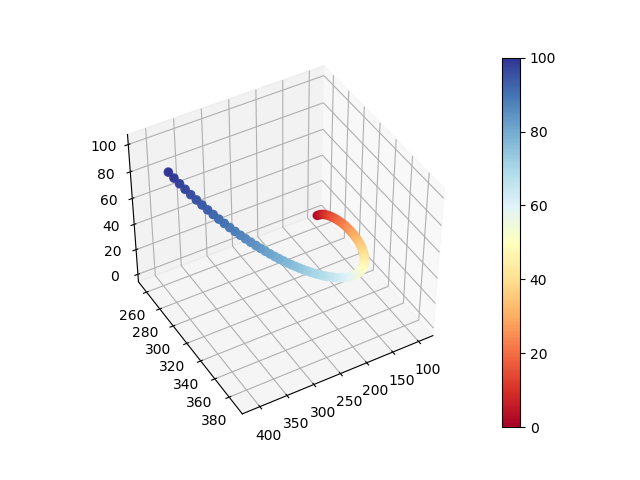
\includegraphics[width=10cm,height=9cm]{2001_0.png}
  \caption{3D图}
\end{figure}
\begin{figure}[H]
 \centering
  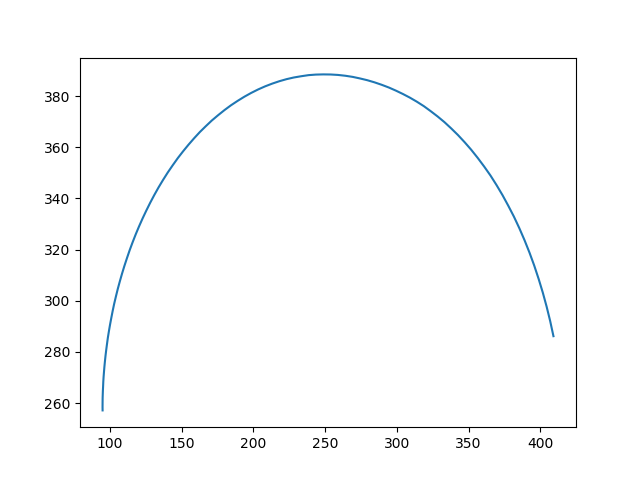
\includegraphics[width=10cm,height=9cm]{2001_1.png}
  \caption{x-y}
\end{figure}
\begin{figure}[H]
 \centering
  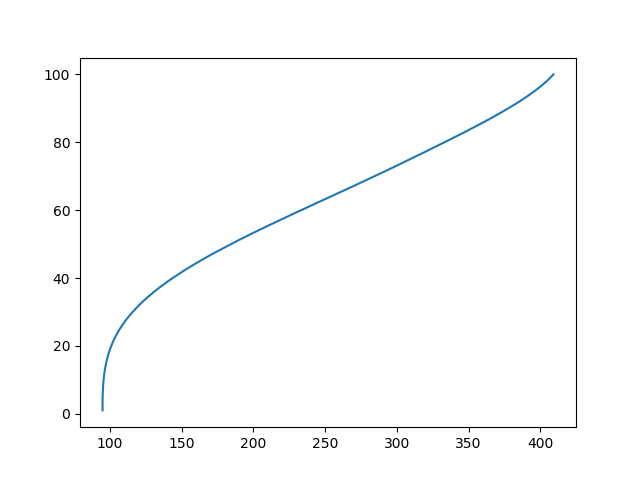
\includegraphics[width=10cm,height=9cm]{2001_2.png}
  \caption{x-z}
\end{figure}
\begin{figure}[H]
 \centering
  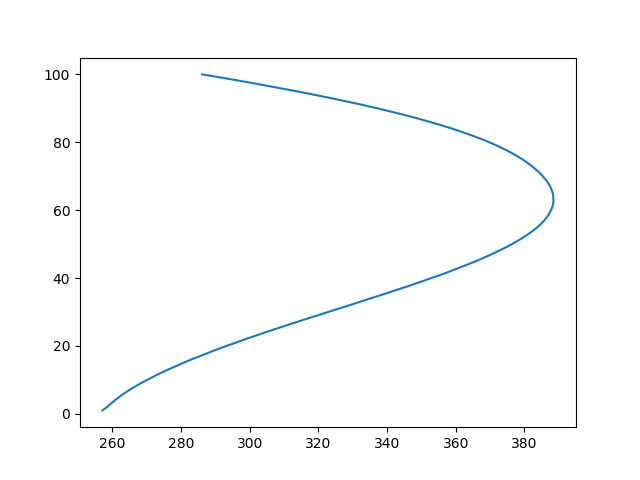
\includegraphics[width=10cm,height=9cm]{2001_3.png}
  \caption{y-z}
\end{figure}
\begin{figure}[H]
 \centering
  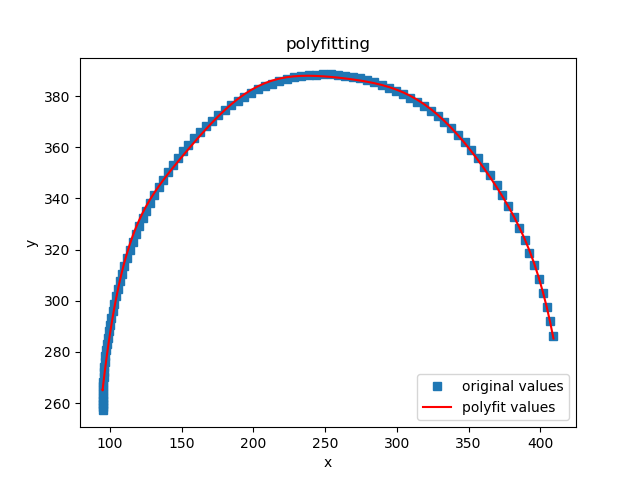
\includegraphics[width=10cm,height=9cm]{2001_4.png}
  \caption{拟合图像1}
\end{figure}
\begin{figure}[H]
 \centering
  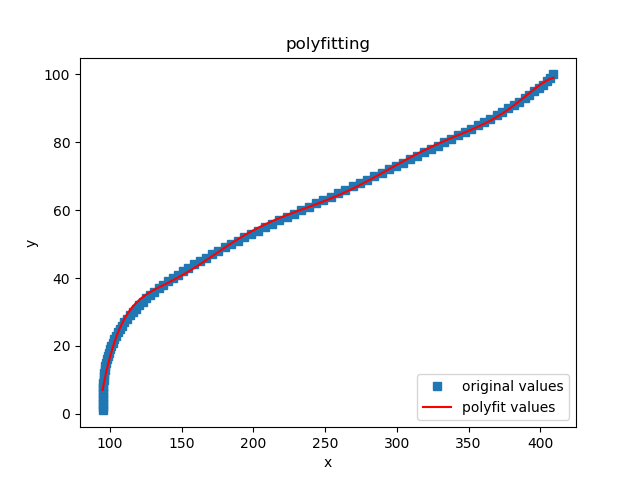
\includegraphics[width=10cm,height=9cm]{2001_5.png}
  \caption{拟合图像2}
\end{figure}


读取图像后,使用kmeans算法求出其中心点,然后进行拟合。


得到参数方程为:

$$
y=-7.17 \times 10^{(-16)} x^8 +1.488 \times10^{-12} x^7-1.322\times 10^{-9} x^6
$$
$$
+6.554 \times 10^{-7} x^5 -0.0001988 x^4 +0.0373 x^3-4.276 x^2+274x-7214
$$

$$
z=-3.777 \times 10^{(-16)} x^8 +7.931 \times10^{-13} x^7-7.115\times 10^{-10} x^6
$$
$$
+3.556\times 10^{-7} x^5 -0.0001081 x^4 +0.02044 x^3-2.345 x^2+274x-4025
$$

\newpage
\section*{致谢}
感谢刘保东教授和窦金峰学姐一学期来的辛勤指导。

通过对数值计算课程的学习,我学会了用计算机能够更好的解决数学问题。在本门课程实验中,我使用 PYTHON 对数学领域的常用算法进行了学习和编程实现,并进行了误差分析。进行完实验的学习之后,我对计算机和数学之间的联系理解的更加透彻,为以后的科研之路打下了良好的基础。

\end{document}
